%%%%%%%%%%%%%%%%%%%%%%%%%%%%%%%%%%%%%%%%%%%%%%%%%%%%%%%%%%%%%%%
%% OXFORD THESIS TEMPLATE

% Use this template to produce a standard thesis that meets the Oxford University requirements for DPhil submission
%
% Originally by Keith A. Gillow (gillow@maths.ox.ac.uk), 1997
% Modified by Sam Evans (sam@samuelevansresearch.org), 2007
% Modified by John McManigle (john@oxfordechoes.com), 2015
%
% This version Copyright (c) 2015-2023 John McManigle
%
% Broad permissions are granted to use, modify, and distribute this software
% as specified in the MIT License included in this distribution's LICENSE file.
%

% I've (John) tried to comment this file extensively, so read through it to see how to use the various options.  Remember
% that in LaTeX, any line starting with a % is NOT executed.  Several places below, you have a choice of which line to use
% out of multiple options (eg draft vs final, for PDF vs for binding, etc.)  When you pick one, add a % to the beginning of
% the lines you don't want.


%%%%% CHOOSE PAGE LAYOUT
% The most common choices should be below.  You can also do other things, like replacing "a4paper" with "letterpaper", etc.

% This one will format for two-sided binding (ie left and right pages have mirror margins; blank pages inserted where needed):
\documentclass[a4paper,twoside]{ociamthesis}
% This one will format for one-sided binding (ie left margin > right margin; no extra blank pages):
%\documentclass[a4paper]{ociamthesis}
% This one will format for PDF output (ie equal margins, no extra blank pages):
%\documentclass[a4paper,nobind]{ociamthesis} 

%%%%% SELECT YOUR DRAFT OPTIONS
% Three options going on here; use in any combination.  But remember to turn the first two off before
% generating a PDF to send to the printer!

% This adds a "DRAFT" footer to every normal page.  (The first page of each chapter is not a "normal" page.)
\fancyfoot[C]{\emph{DRAFT Printed on \today}}  

% This highlights (in blue) corrections marked with (for words) \mccorrect{blah} or (for whole
% paragraphs) \begin{mccorrection} . . . \end{mccorrection}.  This can be useful for sending a PDF of
% your corrected thesis to your examiners for review.  Turn it off, and the blue disappears.
\correctionstrue


%%%%% BIBLIOGRAPHY SETUP
% Note that your bibliography will require some tweaking depending on your department, preferred format, etc.
% The options included below are just very basic "sciencey" and "humanitiesey" options to get started.
% If you've not used LaTeX before, I recommend reading a little about biblatex/biber and getting started with it.
% If you're already a LaTeX pro and are used to natbib or something, modify as necessary.
% Either way, you'll have to choose and configure an appropriate bibliography format...

% The science-type option: numerical in-text citation with references in order of appearance.
\usepackage[style=numeric-comp, sorting=none, backend=biber, doi=false, isbn=false]{biblatex}


% \usepackage[style=authoryear, sorting=nyt, backend=biber, maxcitenames=2, useprefix, doi=false, isbn=false]{biblatex}
\newcommand*{\bibtitle}{References}

% This makes the bibliography left-aligned (not 'justified') and slightly smaller font.
\renewcommand*{\bibfont}{\raggedright\small}

% Change this to the name of your .bib file (usually exported from a citation manager like Zotero or EndNote).
\addbibresource{references.bib}


% Uncomment this if you want equation numbers per section (2.3.12), instead of per chapter (2.18):
%\numberwithin{equation}{subsection}


%%%%% INCLUDING PACKAGES
\usepackage{subfig}
\usepackage{graphicx}
\usepackage{algorithm}
\usepackage{algpseudocode}

%%%%% THESIS / TITLE PAGE INFORMATION
% Everybody needs to complete the following:
\title{Title}
\author{Neil Natarajan}
\college{New College}

% Master's candidates who require the alternate title page (with candidate number and word count)
% must also un-comment and complete the following three lines:
%\masterssubmissiontrue
%\candidateno{933516}
%\wordcount{28,815}

% Uncomment the following line if your degree also includes exams (eg most masters):
%\renewcommand{\submittedtext}{Submitted in partial completion of the}
% Your full degree name.  (But remember that DPhils aren't "in" anything.  They're just DPhils.)
\degree{Doctor of Philosophy}
% Term and year of submission, or date if your board requires (eg most masters)
\degreedate{Trinity 2024}


%%%%% YOUR OWN PERSONAL MACROS
% This is a good place to dump your own LaTeX macros as they come up.

% To make text superscripts shortcuts
	\renewcommand{\th}{\textsuperscript{th}} % ex: I won 4\th place
	\newcommand{\nd}{\textsuperscript{nd}}
	\renewcommand{\st}{\textsuperscript{st}}
	\newcommand{\rd}{\textsuperscript{rd}}

%%%%% THE ACTUAL DOCUMENT STARTS HERE
\begin{document}



%%%%% CHOOSE YOUR LINE SPACING HERE
% This is the official option.  Use it for your submission copy and library copy:
\setlength{\textbaselineskip}{22pt plus2pt}
% This is closer spacing (about 1.5-spaced) that you might prefer for your personal copies:
%\setlength{\textbaselineskip}{18pt plus2pt minus1pt}

% You can set the spacing here for the roman-numbered pages (acknowledgements, table of contents, etc.)
\setlength{\frontmatterbaselineskip}{17pt plus1pt minus1pt}

% Leave this line alone; it gets things started for the real document.
\setlength{\baselineskip}{\textbaselineskip}


%%%%% CHOOSE YOUR SECTION NUMBERING DEPTH HERE
% You have two choices.  First, how far down are sections numbered?  (Below that, they're named but
% don't get numbers.)  Second, what level of section appears in the table of contents?  These don't have
% to match: you can have numbered sections that don't show up in the ToC, or unnumbered sections that
% do.  Throughout, 0 = chapter; 1 = section; 2 = subsection; 3 = subsubsection, 4 = paragraph...

% The level that gets a number:
\setcounter{secnumdepth}{2}
% The level that shows up in the ToC:
\setcounter{tocdepth}{2}


%%%%% ABSTRACT SEPARATE
% This is used to create the separate, one-page abstract that you are required to hand into the Exam
% Schools.  You can comment it out to generate a PDF for printing or whatnot.
% \begin{abstractseparate}
% 	In a globalised world, scholarship programs face pressures to select the ``best'' applicants fairly across regions, but current low-tech selection processes struggle to meet this burden. To address this, we studied two global scholarship programs, exploring data-driven Decision Support Tools (DSTs) for selection. One program was interested in utilising existing AI tools wherever possible. We explored using existing post-hoc explainable AI (xAI) tools as DSTs in a variety of contexts and using existing detection software as DSTs to understand generative AI (genAI)'s role in essays. We developed the \emph{Decision Matrix} framework, categorising decisions by \emph{stage} (\emph{in-process} or \emph{ex-post}) and \emph{stakes} (\emph{high} or \emph{low}), and applied it to assess both technologies as DSTs. Both proved ineffective for \emph{in-process} decisions and useful \emph{ex-post}.

To design a DST for \emph{in-process} decision-making, we engaged in participatory design with both programs, focusing on diversity considerations in selection. Six prototypes were created, with practitioners showing eagerness to use them across the \emph{Decision Matrix}. To validate this enthusiasm, we implemented one design as a technology probe and evaluated its impact. The selected cohort's diversity and performance improved, demonstrating the tool's ability to support high-stakes \emph{in-process} decisions.

Our findings highlight the need for data-driven and AI-based DSTs across the \emph{Decision Matrix}. We propose \emph{Selection-Oriented AI}, focused on the pro-social goals of selection. We conclude with a call for AI-driven DSTs that balance practitioners' needs while optimising selection outcomes for social benefit. % Create an abstract.tex file in the 'text' folder for your abstract.
% \end{abstractseparate}


% JEM: Pages are roman numbered from here, though page numbers are invisible until ToC.  This is in
% keeping with most typesetting conventions.
\begin{romanpages}

% JEM: By default, this template uses the traditional Oxford "Belt Crest". Un-comment the following
% line to use the newer, "Blue Square" logo:
% \renewcommand{\crest}{{
\includegraphics[width=4.2cm, height=4.2cm]{figures/newlogo.pdf}}}

% Title page is created here
\maketitle

%%%%% DEDICATION -- If you'd like one, un-comment the following.
%\begin{dedication}
%This thesis is dedicated to\\
%someone\\
%for some special reason\\
%\end{dedication}

%%%%% ACKNOWLEDGEMENTS -- Nothing to do here except comment out if you don't want it.
\begin{acknowledgements}
 	I would like to thank my advisors Reuben Binns and Nigel Shadbolt: Reuben, for his constant dedication to his students and willingness to run with any idea I came up with; Nigel, for his clear framing and pointed critiques. I would also like to thank my colleagues in Oxford Computer Science's HCAI theme, with special thanks to Sruthi, Ulrik, Jake, and Thomas. I would like to thank my family for their support and my friends for my sanity.
\end{acknowledgements}

%%%%% ABSTRACT -- Nothing to do here except comment out if you don't want it.
\begin{abstract}
	In a globalised world, scholarship programs face pressures to select the ``best'' applicants fairly across regions, but current low-tech selection processes struggle to meet this burden. To address this, we studied two global scholarship programs, exploring data-driven Decision Support Tools (DSTs) for selection. One program was interested in utilising existing AI tools wherever possible. We explored using existing post-hoc explainable AI (xAI) tools as DSTs in a variety of contexts and using existing detection software as DSTs to understand generative AI (genAI)'s role in essays. We developed the \emph{Decision Matrix} framework, categorising decisions by \emph{stage} (\emph{in-process} or \emph{ex-post}) and \emph{stakes} (\emph{high} or \emph{low}), and applied it to assess both technologies as DSTs. Both proved ineffective for \emph{in-process} decisions and useful \emph{ex-post}.

To design a DST for \emph{in-process} decision-making, we engaged in participatory design with both programs, focusing on diversity considerations in selection. Six prototypes were created, with practitioners showing eagerness to use them across the \emph{Decision Matrix}. To validate this enthusiasm, we implemented one design as a technology probe and evaluated its impact. The selected cohort's diversity and performance improved, demonstrating the tool's ability to support high-stakes \emph{in-process} decisions.

Our findings highlight the need for data-driven and AI-based DSTs across the \emph{Decision Matrix}. We propose \emph{Selection-Oriented AI}, focused on the pro-social goals of selection. We conclude with a call for AI-driven DSTs that balance practitioners' needs while optimising selection outcomes for social benefit.
\end{abstract}

%%%%% MINI TABLES
% This lays the groundwork for per-chapter, mini tables of contents.  Comment the following line
% (and remove \minitoc from the chapter files) if you don't want this.  Un-comment either of the
% next two lines if you want a per-chapter list of figures or tables.
\dominitoc % include a mini table of contents
%\dominilof  % include a mini list of figures
%\dominilot  % include a mini list of tables

% This aligns the bottom of the text of each page.  It generally makes things look better.
\flushbottom

% This is where the whole-document ToC appears:
\tableofcontents

% Uncomment to generate a list of figures:
% \listoffigures
% 	\mtcaddchapter

% \mtcaddchapter is needed when adding a non-chapter (but chapter-like) entity to avoid confusing minitoc

% Uncomment to generate a list of tables:
%\listoftables
%	\mtcaddchapter

%%%%% LIST OF ABBREVIATIONS
% This example includes a list of abbreviations.  Look at text/abbreviations.tex to see how that file is
% formatted.  The template can handle any kind of list though, so this might be a good place for a
% glossary, etc.
% First parameter can be changed eg to "Glossary" or something.
% Second parameter is the max length of bold terms.
\begin{mclistof}{List of Abbreviations}{3.2cm}
    \item[AI] Artificial Intelligence
    \item[xAI] Explainable Artificial Intelligence
    \item[DEI] Diversity, Equity, and Inclusion.
    \item[IAI] Interpretable Artificial Intelligence
    \item[DST] Decision Support Tool
    \item[HitL] Human in the Loop 
    \item[IAIDST] Interpretable, Artificially Intelligent Decision Support Tool
    \item[TI] Talent Identification 
\end{mclistof}
See Appendix \ref{app:terminology} for definitions of terms used in this Thesis, including these abbreviations.

% The Roman pages, like the Roman Empire, must come to its inevitable close.
\end{romanpages}


%%%%% CHAPTERS
% Add or remove any chapters you'd like here, by file name (excluding '.tex'):
\flushbottom
% \begin{savequote}[8cm]
% \textlatin{Neque porro quisquam est qui dolorem ipsum quia dolor sit amet, consectetur, adipisci velit...}

% There is no one who loves pain itself, who seeks after it and wants to have it, simply because it is pain...
%   \qauthor{--- Cicero's \textit{de Finibus Bonorum et Malorum}}
% \end{savequote}

\chapter{\label{ch:intro}Introduction} 

\minitoc

Since early theorising about Artificial Intelligence (AI), experts have noted the transformative potential of such technology. Now, with the popular advent of Machine Learning (ML) models and transformer architecture in particular, we see rapid mass-market adoption of a variety of AI tools. In many fields which deal with sensitive decision-making, this adoption introduces new ethical challenges. In the fields of talent and Talent Identification (TI) in particular, many of these ethical challenges centre on decision tool interpretability; diversity, equity, and inclusion (DEI); and applicant usage of generative AI. In this section, we lay out the case for the application of AI systems (specifically interpretable AI decision assistants) to these issues in TI, paying special attention to the potential pitfalls and broader implications of our proposal.

\section{A Brief Account of Talent Identification, its Adoption of Artificial Intelligence, and Challenges Arising}
(To-do)
% Intro needs a sociological account of talent identification. What is it? How does it differ from recruitment? What niche within TI do I focus on? I talk about this a bit in the organisation discussion but should go into greater detail here.

\section{Motivation}
(To-do) This is where I explain why I'm doing this research. I explain why care about talent identification and how IAIDSTs can solve problems here. I respond to the notion that we should simply not use AI here, and highlight problems in the field already. I explain why this is a problem for Computer Science as well as for Talent Science (tl;dr: additional reasons to care about things xai overlooks because of the application domain)

\section{Partner Organisations}
(To-do) Describe the two organisations partnered with for this research.

\section{Contributions}
In this thesis, we make a number of theoretical, technical and practical contributions. These are:

\begin{itemize}
    \item We articulate where talent identification experts should use IAIDSTs to assist in their decision-making, and which IAI systems are appropriate for which purposes
    \item We apply research-through-design methods to talent identification to produce a novel approach to the creation of human-centric selection tooling
    \item We develop a novel method for visualising and understanding cohort-level decisions surrounding diversity called the Selection Possibility Frontier
    \item We further implement a novel algorithm for approximating the Selection Possibility Frontier
    \item We produce several qualitative, quantitative, and mixed-modal datasets relating to talent identification
    \item We demonstrate a yet-undemonstrated risk associated with naive application of post-hoc explainability to a range of problems
    \item We demonstrate the utility and limitation of detection tools for generative-AI-written essays in a scholarship context, and explore implications for scholarship programs
\end{itemize}

\section{Thesis Structure}
In this chapter, we explore our motivation for focusing on the application of IAIDSTs to talent identification, enumerate our contributions, and provide an account of challenges talent identification. Among these challenges, we focus the remainder of this thesis on three: limited human understanding of the AI tools, limited ability to consider diversity, and the risks of applicant usage of generative AI.

In Chapter \ref{ch:background}, we provide a background on the field of talent identification, the field of explainable AI, and the field of diversity, equity, and inclusion; we further explore intersections between these fields of research and identify gaps in the literature. Chapters \ref{ch:xailimitations} and \ref{ch:usingxai} explore our first challenge: limited human understanding of the AI tools. In Chapter \ref{ch:xailimitations}, we explore the limitations of popular xAI methods in the context of talent identification. In Chapter \ref{ch:usingxai}, we explore the use of SHAP explanations in the context of talent identification. Chapters \ref{ch:iaicasestudy} and \ref{ch:spf}  address challenges related to consideration of diversity in TI. In Chapter \ref{ch:iaicasestudy}, we present a participatory design study, which aims to use IAIDSTs to help TI professionals account for diversity. In Chapter \ref{ch:spf} we implement one of the designs from Chapter \ref{ch:iaicasestudy}. Chapter \ref{ch:studentuse} attempts to mitigate the risks of applicant usage of generative AI. It explores the use of generative AI detection tools as DSTs in the context of talent identification. Finally, in Chapter \ref{ch:discussion}, we discuss our design recommendations, note limitations of our approach, and conclude.

\section{Publications}

\begin{itemize}
    \item \textcite{natarajan_trust_2023} Trust Explanations to do What They Say
    \item \textcite{...} `You Trust Me, But Should You?': Misleading Explanations of AI Outputs
\end{itemize}
% \begin{savequote}[8cm]
% \textlatin{Neque porro quisquam est qui dolorem ipsum quia dolor sit amet, consectetur, adipisci velit...}

% There is no one who loves pain itself, who seeks after it and wants to have it, simply because it is pain...
%   \qauthor{--- Cicero's \textit{de Finibus Bonorum et Malorum}}
% \end{savequote}

\chapter{\label{ch:background}Background} 
In this chapter we examine: new advancements in  IAI, open problems in TI and their existing solutions, and human-centric methodologies that might help us applying AI to TI. We first engage in a survey of the field of IAI, including the types of articles prevalent in the field, the prominent paradigms for interpretability and explanation, and several key concepts in the development of new algorithms. Next, we examine open problems in diverse, equitable, and inclusive TI and note pre-existing solutions from prior works. Finally, we examine human-centred methodologies that we may draw on in crafting our own solutions. We further note that some problems are not well-suited to resolution through explanation, and suggest a variety of other solutions that could be attempted in address of these problems.

\minitoc

\section{Interpretable Artificial Intelligence}
\subsection{Types of IAI Publications}

The field of IAI can, broadly, be divided into four main bodies of research: reviews, methods, notions, and evaluations \cite{vilone_explainable_2020}. Review articles are either systematic investigations or literature reviews. Method articles introduce new explanation methods. Notion articles focus on defining notions or concepts related to explainability. Evaluation articles evaluate existing notions or paradigms.

\subsubsection{Review Articles}
Review articles offer meta-commentary on other articles listed below. A review article is so-characterised because its primary contribution is one of aggregation. Thus, a review article might also be a method, notion, or evaluation article, so long as it primarily draws from these articles. This paper is, primarily, a review article.

\subsubsection{Method Articles}
In most method articles, the task of explanation is taken to be fairly well-defined, and the research questions deal in how to most effectively generate that explanation. 

Consider two particular method articles: SHAP explanations, introduced by \textcite{lundberg_unified_2017}, and counterfactual explanations, introduced by \textcite{wachter_counterfactual_2017}. In both papers, we see heavy treatment of the mathematical properties of the explanation algorithm introduced. However, we see relatively light treatment of what the authors take to be a good explanation or proposed use cases for the novel methods. These concepts are instead the domain of notion articles.

\subsubsection{Notion Articles}
Where method articles deal with individual methods, notion articles deal with theory underlying a variety of methods. For example, \textcite{miller_explanation_2017} discussion of the importance of principles of explanation from the social sciences is a notion article.

\subsubsection{Evaluation Articles}
Evaluation articles consider which notions and methods are best-suited to produce the best explanations. Evaluations of method articles, in particular, often compare them to notions introduced elsewhere, and where critiques are found, they are often critiques that the method fails to meet a standard set by the notion.

For the two method articles discussed above, we present two evaluation articles: \textcite{kumar_problems_2020} evaluation of the SHAP method, and \textcite{barocas_hidden_2020} evaluation of counterfactual explanations. Both articles rely on similar notions regarding the purpose of explanations, and critique the methods for failing to adhere to a notion. For instance, \textcite{barocas_hidden_2020} assume that counterfactual explanations are given to provide users actionable information. Similarly, \textcite{kumar_problems_2020} argue that SHAP cannot be used to inform users' actions.

\subsection{A Taxonomy of IAI Methods}
AI model explanations can broadly be categorised into two subgroups: intrinsically interpretable models and post-hoc explanations \cite{molnar_interpretable_2019}. Though intrinsically interpretable models offer explanations and are meaningfully classed as forms of “interpretable AI”, they do not make use of the major developments in “explainable AI” \cite{molnar_interpretable_2019}, since they are already interpretable.

Post-hoc methods can be further separated into global methods, which explain entire models, and local methods, which explain individual decisions \cite{molnar_interpretable_2019}. When assessing explanation methods, one can distinguish between local tests and global tests of model explanations \cite{molnar_interpretable_2019}. Local tests concentrate on the impact of the explanations at the level of a single prediction, global tests focus on the impact of explanations on overall model trust.

Rather than delineating between intrinsic and post-hoc or global and local, we could instead delineate by output type \cite{friedrich_taxonomy_2011}. Some interpretability devices offer feature importance statistics. Others offer explanations by contrast to another datapoint. Yet others offer rules that guide decision-making in regard to an individual case case.

\subsection{Use Case}
Consider the following potential use cases for xAI methods: to evaluate whether the AI is operating as intended, to examine an AI for bias and unfairness, to provide recourse, to provide a rule that would guarantee equality. This list is not exhaustive, and yet, even for these three use cases, explanations that satisfy some will not satisfy others \cite{natarajan_trust_2023}.

\subsection{Theories of Explanation}
In deciding which type of explanation will best suit a particular use case, we must consider the theory of explanation that underlies the explanation, and the desiderata that that theory demands of its explanations.

\textcite{miller_explanation_2017} summarises key findings from Social Sciences related to explanation. \textcite{miller_explanation_2017} works from a causal theory of explanation; he outlines and examines the theory, noting challenges to it, but does not consider a rejection of the theory. According to the theory, explanations are sought in response to counterfactual cases, i.e. the question asked is not of the form "Why \textit{P}" but rather "Why \textit{P} instead of \textit{Q}" \cite{miller_explanation_2017}. Such counterfactual theories of causality all argue that cause is a matter of what would have happened if the cause had not happened. Though they disagree on precisely how to model these counterfactual cases, many leading philosophical theories of causality agree that causality is best understood in terms of counterfactuals. Hume modeled these counterfactuals in terms of causes and events: in actuality, cause $C$ caused event $E$ to occur; but if cause $C'$ had replaced cause $C$, $E$ would not have occurred. We can call this sort of counterfactual a cause-counterfactual \cite{miller_explanation_2017}. Under this conception, explanations should present cause-counterfactuals as clearly as possible.

\textcite{miller_explanation_2017} also argues that explanations should be contrastive and selective. Contrastive explanations make use of counterfactuals, but these counterfactuals are not cause-counterfactuals. Instead, they are event-counterfactuals. In other words, contrastive explanations consider alternative events $E'$, and explain the data $E$ in relation to $E'$. Selective explanations, on the other hand, are ones that do not consist of a complete cause, but rather select one or two causes from the complete cause. 

\textcite{miller_explanation_2017} presents a powerful application of a theory of explanation to the field of xAI. However, causal theories of explanation are far from the only type of explanatory theories. Indeed, as we noted above with numerical evidence, there are theories of explanation who's desiderata contradict those of \textcite{miller_explanation_2017}'s causal theory \cite{woodward_scientific_2021}. 

In what follows, I present \textcite{woodward_scientific_2021}'s theory, the statistical relevance model of explanation. The statistical relevance theory rests heavily on the notion of statistical relevance. For events $A$, $B$, and $C$, we say $C$ is statistically relevant to $B$ in $A$ if and only if $P(B | A \land C) \neq P(B | A)$. I.e., an explanation is a member $C_i$ of a homogeneous partition $C$ of properties: that is, a set of properties that are exclusive and exhaustive of $A$, where there are no statistically relevant properties $D$ to $B$ in $A \land C_i$. The explanation also consists of $P(B | A)$, the probability $P(B | A \land C_i)$ of each cell withing the partition, and which of the $C_i$ contains the desired point to be explained, $x$ \cite{woodward_scientific_2021}.

On both accounts , explanations have an explainer and an explainee. Explanations in everyday use are an interaction. Unlike most modern algorithmic explanation methods, an explanation given by a human is often given in the form of a conversation. Thus, it obeys the rules of communication using language. In other words, these explanations are social. We may therefore apply theories governing social interactions, such as \textcite{Grice_1975}'s conversational maxims, to explanations \cite{miller_explanation_2017}.

\textcite{Grice_1975}'s four categories of conversational maxims are: quality, quantity, relation, and manner. That is, the quality of information conveyed in a cooperative conversation should be high (information should be likely and justifiable). The quantity of information should be neither too little nor too much. The information should be related to the conversation. The information should be conveyed in an appropriate manner. Note that the quantity bounds overlap quite heavily with selectivity.

\subsection{Trust}
Another important notion related to xAI is trust. Indeed, much of the xAI literature suggests that the purpose of xAI is to increase trust in AI. This is apparent from the titles of canonical papers in the field, such as \textcite{ribeiro_why_2016} and \textcite{pieters_explanation_2011}. So what does it mean to trust an AI system? A basic philosophical analysis of what trust consists in (in the general, non-algorithmic sense) is as follows: $A$ trusts $B$ if and only if $A$ believes that $B$ will act in $A$'s best interest, and $A$ accepts vulnerability to $B$'s actions \cite{jacovi_formalizing_2021}. Moreover, trust often does not have a blanket scope; typically, $A$ will trust $B$ regarding some particular actions or motivations.

An important distinction here can be drawn between whether someone or something is trusted and whether that trust is warranted; i.e. it is worthy of trust \cite{hardin_trust_2002}. In the context of AI, according to \textcite{jacovi_formalizing_2021}, we should only ever trust AI systems to fulfil their contracts, but some AI systems are not worthy of even this trust. Ideally, trust in a system should relate directly to that system's trustworthiness – we should place trust in any system when it warrants trust, but should not place unwarranted trust in any system. The problem of appropriately calibrating trust, however, is yet unsolved.

There are many methods that aim to calibrate trust in an AI algorithm. We could give some access to the patterns that distinguish correct and incorrect cases. The better some end-user is able to distinguish these, the better they know when they can trust the model to be correct. Knowledge of the performance of a model grants access to the patterns distinguishing correct and incorrect cases. Facts about the bias of the model grant access as well, as does information about the performance of the model on a subset of data. Explanations can be seen as one way of imparting such information. Because of this, algorithm explanations allow explainees to determine when an algorithm is trustworthy. 

\subsection{Relevant Evaluations of XAI}
There is a growing body of studies that empirically evaluate xAI methods. In some cases, an xAI method is evaluated not with human subject experiments but rather with some formally defined proxy for interpretability \cite{doshi-velez_towards_2017}. However, most evaluations involve humans using an AI system to perform some task, and the effect of an xAI method on task performance is measured.  For our purposes, namely the measurement of end-user trust and reliance, we need to measure lay people using a system in a simplified but realistic task.

It should also be noted that there is no standard evaluation or set of benchmarks explainability methods are judged by \cite{doshi-velez_towards_2017}. Indeed, though there are proposed methods for evaluating attribution-based explanations and model-based explanations, there are none for evaluating example-based explanations \cite{markus_role_2021}. As a result, there exist a variety of study designs, conditions, and variables measured by human-centred evaluation papers. We list some such studies here.

\textcite{ford_play_2020} run a study where they examine the impact of post-hoc explanations-by-example and error-rates on people's perceptions of a black-box classifier. They show that case-based explanations lead participants to perceive miss-classifications as more correct. In the case of their study, a case-based explanation is a series of three important data points in the training of the model (in other words, an “influential instances” explanation). They also show that classifiers with higher error rates lead participants to perceive the models as less trustworthy. They show participants a series of machine classifications of the MNIST dataset, where the model either correctly labels the data or commits an alternate labelling error. They then task the participants with rating correctness and reasonableness of each classification on a 5-point scale. Finally, at the end, the participants filled out global correctness and reasonableness, alongside global trust forms. The design was a 2x3 design, with explanations present or absent, and three accuracy levels. Participants report miss-classifications as being more correct when given a case-based explanation. They did not find significant findings for reasonableness, trust, or satisfaction across explanation-present or explanation-absent conditions. They use a MANOVA design to account for differences across conditions, but use a between-subjects design \cite{ford_play_2020}. 

\textcite{jacobs_how_2021} run a study in the medical diagnosis context, where participants are given a vignette of a patient and, in the experiment condition, a recommended treatment list and explanation. Participants were asked to make an antidepressant treatment selection, to rate their confidence, and to indicate the utility of the model on their decision (it appears on a 5-point scale). The study had statistically significant results only with respect to accuracy (measured as an average of 0s and 1s), not confidence or perceived utility. In the accuracy case, this indicated that an algorithmically generated treatment list, when wrong, would mislead the participants and lower their accuracy. In the confidence and utility cases, this would indicate either that accuracy is affected, but not confidence or utility, or that the Likert scale measurement method used in Jacobs et al.'s study is a weaker measurement tool than the accuracy. Furthermore, these findings are not isolated to the explanation. Rather, Jacobs et al. consider the recommendation and the explanation together. For example, they find that feature-based explanations, paired with incorrect recommendations, lowered accuracy compared to the baseline condition (no recommendation) \cite{jacobs_how_2021}. 

\textcite{bansal_does_2021} perform another similar study, looking at human-AI cooperation in a context where they have comparable performance. They use sentiment classification as their task. Furthermore, they measure effects with a variety of explanations. They find that explanations inspire increased trust in AI systems regardless of the correctness of the model. As explanation, they use a highlighting of the top predicted sentiment classes, alongside a highlighting of important words. Finally, they test expert-generated explanations to serve as an upper bound, as they found that humans were often confused when machine explanations made little sense. They note that explanations make the user more likely to have high accuracy when the AI is correct, but more likely to have low accuracy when the AI is incorrect. This would indicate that AI recommendations with explanations are capable of fostering mistrust, as they foster both overtrust and under trust \cite{bansal_does_2021}.

\textcite{mohseni_trust_nodate} measure user trust in an AI fake news detection system over time. They design a study in which users are shown true and fake news articles. The users are asked at three different points (each one additional third through the study) what their perceived accuracy of the explainable AI system is. They had three different conditions, segmented by type of explanation. There was a baseline condition with no explanation and two xAI conditions. They show that the user trust can be clustered into five profiles: consistent overtrust, consistent under trust, consistent trust, trust gains continually, and trust decreases continually. They show that more participants from the no explanation and attribute explanation conditions were consistently gaining trust, and that more participants from the attention explanation condition overshot their second perceived accuracy measurement \cite{mohseni_trust_nodate}.

\section{Open Problems in Diverse, Equitable, and Inclusive Talent Identification}
We highlight several open problems in TI that touch on concerns of DEI. To begin with, we define DEI alongside related concepts such as JEDI, EDI, DEIB, and IDEA. Then we spotlight the potential equity challenges posed by the integration of DSTs into TI workflows. In particular, we note that any bias and fairness issues built into a DST will create bias and fairness issues for the corresponding TI workflow. However, we note that problems of bias and fairness in TI exist even in the absence of DSTs. We move on to discuss fairness issues posed by applicant use of Generative AI. Finally, we note that TI professionals consistently struggle to balance selecting talented individuals with constructing a diverse cohort and note the implications for equity that this struggle brings.  

\subsection{Bias}
\subsubsection{The Problem of Bias}
We can define the problem of bias as the liability of systems to exhibit different behaviour on groups segregated across a “special” partition. “Special” here refers to partitions across protected classes, or partitions across which we would expect a system to perform equally. For example, gender and race are usually special partitions in the context of talent identification, but academic ability and teachability are not. 

To illustrate the issue of bias in AI systems, we turn to \textcite{mattu_how_nodate}'s analysis of the COMPAS system. The COMPAS system was an expert-system used to predict recidivism of criminals in the US. When defendants accused of crimes were booked in jail, they responded to a COMPAS questionnaire. These answers were then fed into the COMPAS software to produce predictions of the “Risk of Recidivism” and “Risk of Violent Recidivism.” These predictions were used, among other things, to determine if a defendant could be set bail (as likelihood of reoffence is a significant factor in the setting of bail). When \textcite{mattu_how_nodate} analysed the COMPAS tool's predictions relative to actual recidivism rates, they found that the recidivism predictions had roughly equal accuracy for White and Black defendants, but that, when errors were made, these errors acted in very different directions. That is, the Black defendants were more likely to be falsely predicted to reoffend, and the White defendants were more likely to be falsely predicted to not reoffend. As a result, the implementation of the COMPAS system had significantly greater negative externalities on the Black community than on the White community \cite{mattu_how_nodate}.

\textcite{barocas_big_2016} illustrate how data mining yields exactly this sort of bias. In the example of the COMPAS set, much of this bias comes from the underlying training data, but the software's predictions were, on average, \emph{more} biased than the underlying data, as the process the software used to optimise its predictions exacerbated any biases in the underlying data \cite{barocas_big_2016}.

\subsubsection{How Modifying Training Data Addresses Bias}
In some cases, algorithmic bias introduced via latent biases in the training data can be corrected rather simply by altering training data before the training process. One case of bias arises when one group across a special partition is much smaller than other groups \cite{barocas_big_2016}. Due to this sample size imbalance, optimising for accuracy across the total group leads to overemphasis on accuracy on the large group, and allows for marginal improvements in performance on the larger groups at the cost of performance on the smaller groups. While we might address this problem with explainability methods, in this case, the most straightforward solution rather involves increasing the attention paid to the small groups in training, either by increasing the rate at which we sample from this group, or by increasing the weight applied to each sample \cite{barocas_big_2016}. 

However, though simple, this solution is not always effective. Sometimes, for example, biases are introduced in the content of the training data, rather than their distribution. In this case, heterogenously biases errors in the variable to be predicted induce those same biases in the predictive algorithm. In this case, the solution is to correct the biases in the data itself, but this is often either prohibitively difficult, or outright impossible \cite{barocas_big_2016}. 

\subsubsection{How IAI Addresses Bias}
When bias cannot be removed, it instead might be managed. Where biased behavioural patterns exist in an AI system, simply making these systems more interpretable will not alter these patterns themselves. However, with humans in the loop, spotlighting algorithmic bias might allow humans to address it.

Consider the COMPAS example again, except suppose now that COMPAS implements a counterfactual explanation, which points to a similar hypothetical input that would have a different output. Suppose a defendant has a high calculated risk of reoffense. The actual defendant's race is “black”, but the counterfactual explanation reveals that a similar white defendant would have had a low calculated risk of reoffense. That is, COMPAS is, in this case, clearly discriminating based on race. If this were used in a courtroom setting, a judge might see this information and subsequently choose to disregard the prediction yielded by COMPAS. In this way, an explanation could indicate that an algorithm was biased and encourage scrutiny of that algorithm \cite{mothilal_explaining_2019,wachter_counterfactual_2017}.

Furthermore, in certain special circumstances, implementing techniques from IAI at training time can actually remove bias. For example, we could imagine imposing explanation-based constraints on a model at the time of training. One such constraint would be \textcite{wang_deontological_2020}'s `monotonicity' constraint , which would require that a particular input i relate monotonically to the model's output. Thus, if feature sets X and X' differ only in i such that i in X' is greater than i in X, and M is a model that is monotonic in i, then M(X') should be greater than M(X). This constraint would prevent a model from making decisions that penalise applicants based on, for example, membership in a minority group.

\subsection{Fairness}
\subsubsection{The Problem of Fairness}
Fairness is closely tied to, though still distinct from, Bias. Where bias deals with groups, fairness deals with individuals. We can define the problem of fairness as the liability of AI systems to exhibit different behaviour on different individuals that are similar in relevant dimensions. We can note this follows the given principle, entitled the “similar treatment” principle: if two individuals are similar across relevant dimensions, they should be treated similarly \cite{Fleisher_2021,dwork_fairness_2012}. 

Consider again the COMPAS example. Where the disproportional treatment of groups is a form of bias, an individual decision yielding a false positive in one individual, and a false negative in another individual is a problem of fairness. We can call this form of fairness “Individual Fairness”, and contrast it with other forms of fairness such as statistical parity fairness, where a system is fair if and only if it achieves parity between groups \cite{Fleisher_2021,dwork_fairness_2012}. We focus on individual fairness as a particularly important definition of fairness, and note that statistical parity fairness is more closely bias, as we have defined it. However, note that individual fairness is not a privileged form of fairness. \textcite{Fleisher_2021} argues this, and notes that individual fairness is undesirable when it conflicts with other notions of fairness. Thus, we also note that there are more general notions of fairness that we might address as well.

\subsection{Addressing Fairness}
Much like bias, fairness is not address directly via interpretability alone. Rather, they address fairness indirectly by highlighting unfair uses of AI systems. Indeed, xAI methods that address bias in this manner also address fairness. However, though the notion of individual fairness is not addressed, there are other forms of fairness that can be addressed by xAI methods.

One such method is the presentation of \textcite{ustun_actionable_2019}'s actionable recourse. Suppose some AI system $S$ makes yields some outcome $y$ for some person $P$ represented by feature set $X$. Suppose further that $y$ is an unfavourable outcome for $P$, and $y'$ would have instead been a favourable outcome. Actionable recourse information, in this case, is information that would allow $P$ to change their representation to feature set $X'$ such that $M(X')= y'$. In other words, recourse informs individuals what they would have to change in order to be received more favourably by an AI system. As \textcite{ustun_actionable_2019} argue, the mere presentation of this information makes a system more fair, as the decisions made by this system are accompanied by a means of achieving a more favourable decision, so individuals are always given the opportunity to improve their outcomes.

However, while this creates a form of fairness where individuals' outcomes are less fixed, it does not ensure individual fairness. This is by design – actionable recourse does not handle the differential treatment of similar individuals \cite{ustun_actionable_2019}. Indeed, one might contend, as \textcite{Fleisher_2021} does, that individual fairness is sometimes undesirable, especially when it conflicts with other notions of fairness.

\subsection{Transparency}
\subsubsection{The Problem of Transparency}
The problem of transparency is primarily motivated by the desire of stakeholders in an AI system to understand what a given system does and why. For example, in the above COMPAS example, a defendant may desire to understand why their bail was set where it was. In this case, we might consider it insufficient to simply say that COMPAS was used, as we might desire to understand why COMPAS set the recidivism prediction as it is. For most complicated AI systems, this desire cannot be met outright.

An ancillary concern here is trust. While the COMPAS example is not one in which the defendant need trust the system, there are many potential implementations of AI systems where the system's ability to work is contingent on the user trusting the system. For example, consider a system that analyses patients diagnosed with depression and suggests antidepressants as in \textcite{jacobs_how_2021}. This work is traditionally done by clinicians, but with the assistance of a machine, the work could potentially be made both easier and more accurate. However, these benefits are contingent on the clinicians' appropriate trust in the system assisting them. That is, they should neither blindly trust nor blindly distrust the machine. Rather, they should trust the machine appropriately, relying upon the machine when it is reliable and ignoring it when it is not. In order to achieve this, transparency into the AI system's reasoning process is desirable.

There are, however, times where total transparency is undesirable. Most obviously, scoring algorithms that are completely transparent to their users can be gamed. However, there are other reasons for algorithms to be less-than-transparent to their users. For example, if a system is optimised around a given condition, explaining this reasoning to a decision-maker may make them more likely to override given decisions, which will only lead to a less optimal system.

\subsection{Addressing Transparency}
Unlike bias and fairness, transparency can be directly addressed through explainability methods. Indeed, any explanation of a system or that system's outputs will increase that system's transparency. As such, all explanation will have some impact on transparency. However, this does not imply that explanation constitutes a complete solution to the problem of transparency. 

Consider local explanations such as \textcite{lundberg_unified_2017}'s SHAP and \textcite{ribeiro_anchors_2018}'s Scoped Anchors. Both explanations yield insights into a particular prediction made by a model. However, in their most straightforward application, neither provides transparency into the model in general – rather, they provide transparency into the model in this particular use case. Scoped Anchors, in particular, is designed to give transparency into a single use case – by bounding the given feature with an Anchor, we can replace the model locally with a decision rule \cite{ribeiro_anchors_2018}. SHAP, on the other hand, can be extended to provide transparency into a model in general by taking the average feature importances across the distribution of the training set, yielding feature importances for the model overall \cite{lundberg_unified_2017}.

It is also worth noting that not all explanations yield equivalent forms of transparency. For example, while a question like “why does the model yield a particular prediction in a particular case” is well-answered with Scoped Anchors, it is not well-answered by SHAP \cite{lundberg_unified_2017,ribeiro_anchors_2018}. Evaluations such as those by \textcite{binns_human_2022} and \textcite{rader_explanations_2018} indicate that different forms of explanation answer vastly different questions. Thus, the particular problem of transparency in question will have a strong bearing on what explanation method should be used to solve it.

\subsection{Diversity [WIP]}
[To-do]...

\section{Prior Applications of IAIDSTs to Diverse, Equitable, and Inclusive Talent Identification [WIP]}
We examine other approaches to designing decision support tools for talent identification professionals. We examine computational approaches to fairness here, including the 'similar treatment' principle. We pay special attention to measurements of diversity including the straightforward majority/minority group method and the Entrofy algorithm.

\section{Methodologies [WIP]}
\subsection{Research Through Human-Centered Design}
This section enumerates research-through-design methods and explores relevant method papers. It focuses on the design methodologies employed in building the SHAP algorithm and the SPF algorithm.

\subsection{Quantitative Methods and Statistical Analysis}
This section covers both collecting information from users (i.e., online surveys) and robust statistical analyses applied both to those surveys and to the work in generative AI detection.

\subsection{Qualitative Methods and Thematic Analysis}
This section focuses on running interviews and group thinkaloud sessions. It also covers thematic analysis following Braun and Clarke.


% \begin{savequote}[8cm]
% Alles Gescheite ist schon gedacht worden.\\
% Man muss nur versuchen, es noch einmal zu denken.

% All intelligent thoughts have already been thought;\\
% what is necessary is only to try to think them again.
%   \qauthor{--- Johann Wolfgang von Goethe \cite{von_goethe_wilhelm_1829}}
% \end{savequote}

\chapter{\label{ch:xailimitations}Limitations of Post-Hoc Explainable AI}

\minitoc

\section{Introduction}
Increasingly, decisions affecting the lives of lay people are made by AI algorithms. And while these algorithms may be useful, they can also be dangerous. Users of AI systems desire an understanding of how these systems functions and why they yield the outputs they do, so that they may respond appropriately to the outputs \cite{binns_human_2022}. When AI systems make decisions impacting the user, user insight into the decision-making process allows for recourse \cite{ustun_actionable_2019}. However, when decision-making systems involve both an AI and human component, user insight into AI outputs is crucial in both (1) inducing appropriate reliance or scepticism in the AI as warranted and (2) optimising the overall performance of the decision-making system. This is especially true in high-stakes domains such as healthcare, finance, and criminal justice, where the decisions made by AI systems can have significant consequences for individuals \cite{binns_human_2022,ustun_actionable_2019,wachter_counterfactual_2017}.

The growing field of Explainable Artificial Intelligence (xAI) aims to develop methods for explaining algorithms. While some models are intrinsically interpretable \cite{rudin_interpretable_2021}, many more complicated machine learning algorithms are difficult to interpret. In order to explain these more complex models, various dedicated explanation algorithms have been proposed. Within the field of xAI, post-hoc, model-agnostic explainability methods remain popular due to their flexibility and ease-of-application \cite{molnar_interpretable_2019}. Indeed, the ability of methods like SHAP, LIME, and Scoped Anchors to treat any model as a black-box allows for applications of explainability to models that would be otherwise inscrutable \cite{lundberg_unified_2017,ribeiro_why_2016,ribeiro_anchors_2018}. However, there are several known limitations that can impact their utility as IAIDSTs; in some cases, these limitations undermine the purpose of explanation, or even to deceive and mislead users \cite{wang_transparency_2022}. 

In this Chapter, we explore a disconnect between user trust in an AI system and that system's trustworthiness as a result of post-hoc explainable AI tools. We begin by citing a series of papers yielding this result in a variety of contexts, and proceed to present our own work confirming that this disconnect persists in talent identification tasks. We then identify theories of when and why this disconnect occurs, and propose a series of experiments to test these theories. 

In Chapter \ref{ch:usingxai}, we implement these experiments and present the results.

\section{Trust and Trustworthiness in Explainable AI}
\textcite{jacovi_formalizing_2021} set out rules for trust in an algorithmic context. They set out a basic philosophical analysis of trust (in the general, non-algorithmic sense): A trusts B if and only if A believes that B will act in A's best interest and accepts vulnerability to B's actions. Trust often has limited scope; typically, A will trust B regarding some particular actions or motivations, but not others.

In the context of trust in AI, this definition is only slightly changed. \textcite{jacovi_formalizing_2021} characterise trust in an AI system by two properties: ``the vulnerability of the user, and the ability to anticipate the impact of the AI model's decisions''; \textcite{vereschak_how_2021} similarly isolate three elements: ``trust is linked to a situation of vulnerability and positive expectations, and is an attitude''; \textcite{lee_trust_2004} give a similar definition of trust: ``An attitude that an agent will achieve an individual's goal in a situation characterized by uncertainty and vulnerability''. In all definitions, we see \emph{vulnerability} emerge as a key concept, and we variably also see that trust is characterised by \emph{uncertainty} and \emph{expectations}.

An important distinction here can be drawn between whether someone or something is trusted and whether that trust is well-placed; i.e. it is worthy of trust \cite{hardin_trust_2002}. In the machine context, \textcite{jacovi_formalizing_2021} argue, an algorithm is worthy of trust if and only if there exists some contract that the algorithm promises (or that the algorithm's creators and implementors promise) to uphold. They term this a `contractual' model of trust. We adopt the nomenclature of contractual trust and use it to frame breakdowns in trust in specific post-hoc explanations.

\section{A Series of Concerning Results}
\subsection{The Dangers of Transparency}
It is often assumed in the xAI literature that transparency of AI systems is always desirable \cite{molnar_interpretable_2019,miller_explanation_2017-1}. However, \textcite{wang_transparency_2022} dispel this claim. In particular, they demonstrate how, rather than empowering users and stakeholders, some implementations of algorithmic transparency serve the system's deployers, rather than its users, either through a false sense of understanding or the enforcement of norms and power structures. They examine the USA's FICO credit score, which releases the factors that go into the score, the data sources for these factors, and general guidelines on how these factors are used. They find specific information on the use of these factors lacking, and conclude that, rather than empowering users to debate the ethics of certain decisions, this transparency only serves to enforce certain behaviours among the users \cite{wang_transparency_2022}.

\textcite{ustun_actionable_2019} note a similar danger in transparency. They argue that explanations of AI systems making decisions about at end-users should empower those end users to alter the system's determinations. In particular, they introduce the concept of `Actionable Recourse', which consists of a specific set of actions an end-user can take to change the AI's determination, and demonstrate how to calculate these for linear models. Key to actionable recourse is that the actions an explainee should take in response to the explanation are clear in the explanation \cite{ustun_actionable_2019}.

We extend this concept to the context of IAIDSTs. Explanations aimed at decision-makers need not provide them \emph{recourse}, as decision-makers already posses the ability to override the AI system. However, they should still provide \emph{actionable} information, so that the explanations should contain information relevant to the decision-makers choice of what to do with the machine recommendation.

\subsection{Black Box Explanations Increase User Trust in AI Systems}
A number of studies exploring popular post-hoc, black-box explanation algorithms have found that these methods tend to increase overall user trust in the system being explained \cite{ford_play_2020,jacobs_how_2021,wang_transparency_2022}. 

\textcite{ford_play_2020} explore this effect in the context of a machine decision-maker with a human evaluator. They run a study examining the impact of post-hoc explanations-by-example and error-rates on people's perceptions of a black-box classifier classifying images from the MNIST dataset. They show that presenting `case-based explanations' (a series of three important data points in the training of the model; elsewhere, we term this an `influential instances' explanation and use `case-based' more broadly) lead participants to perceive miss-classifications as more correct \cite{ford_play_2020}.

\textcite{jacobs_how_2021} extend this result to a human-in-the-loop context. They study the effect of machine recommendation on a clinician's ability to select antidepressant treatments, and find that providing clinicians an incorrect algorithmically generated treatment list lowers the accuracy of clinicians' own treatment lists. Notably, they do not isolate this result to the presence of an explanation, but rather demonstrate how two explainable AI systems harm clinician antidepressant selection relative to a placebo group. However, they also find that feature-based explanations mislead clinicians more than heuristic-based explanations. Modern best practices outlined by \textcite{miller_explanation_2017-1} prefer the usage of feature-based explanations, so we find this particularly alarming \cite{jacobs_how_2021}.

\textcite{mccradden_when_2021} responds to \textcite{jacobs_how_2021} questioning the role of accuracy in explanations of IAIDSTs. They note the focus of \textcite{jacobs_how_2021} on improving \emph{accuracy} of the treatment lists, and aim to do this with IAIDSTs. However, though these systems may optimise for accuracy, they notably fail (at least in these specific instances) to facilitate clinicians' ability to \emph{help patients}, which is a clinicians' primary goal \cite{mccradden_when_2021}.

In a broader context, while `helping patients' doesn't describe the goal of all IAIDSTs, neither does `improving accuracy'. And, though increasing decision-maker trust regardless of system veracity may improve overall accuracy, it may hamper the broader goal of the decision-making system.

\subsection{Impacts on Talent Identification}
It should be noted that these effects are not universal. \textcite{mohseni_trust_nodate} measure user trust in an AI fake news detection system over time, and find the profile of the users to be just as important as the type of explanation. Though they demonstrate that different explanatory conditions have differential effects on which profile participants are likely to exhibit, they also cluster trust into five profiles by user: consistent over-trust, consistent under-trust, consistent trust, trust gains continually, and trust decreases continually. These profiles suggest that the same explanations will impact different groups performing different tasks differently. Thus, while an IAIDST may lead clinicians selecting antidepressants astray, it may have no effect (or even the opposite effect) on talent identification tasks \cite{mohseni_trust_nodate}.

In the next section, we undertake a series of experiments to test the implications of these limitations for talent identification.

\section{Misleading Explanations of AI Outputs in Talent Identification}
\subsection{The Studies}
We design two studies to answer the question: ``Can explanations of AI outputs create unwarranted user trust in those outputs?''. In particular, we restrict our research question to tasks familiar to lay people with a well-defined but difficult-to-ascertain ground truth. Furthermore, to help make comparisons to related works, we select tasks common in xAI research. Our two tasks are: \emph{estimating a hypothetical person's salary} based on census information of that individual, and \emph{predicting whether someone will be severely delinquent in making a credit payment}. We use two datasets: the Adult dataset collected in the 1994 US Census and curated by \textcite{kohavi_scaling_1996} and the Give Me Some Credit dataset curated by \textcite{GiveMeSomeCredit}. In both tasks, the participant aims to accurately estimate the dependent variable with the help of the AI system and one of several possible explanations of the AI system's estimate (which is possibly just the confidence rating of the model). More detail on the selection of our tasks can be found in Appendix \ref{app:misleadingexplanations}.

We have preregistered some of the analyses in both of our studies in the OSF registries \cite{natarajan_binns_2022}. In particular, we preregistered the analyses in Subsections \ref{ssec:ttests} and \ref{ssec:anovas} for both tasks. We also preregistered the analyses in Subsections \ref{ssec:hsd-salary} and \ref{ssec:hsd-credit}. Finally, we preregistered the analysis in Subsection \ref{ssec:trust-corr} for the Credit Prediction task only after observing interesting results in the Salary Estimation task.

\subsection{The Model}
In both cases, we construct a model using random forests and three different explanatory conditions. Our random forest classifier achieves 86\% test accuracy on the Adult dataset and 93\% test accuracy on the Give Me Some Credit dataset.

We use three explanatory conditions: SHAP, Anchors, and Confidence. 

More information on the models themselves and the explanatory conditions is provided in Appendix \ref{app:misleadingexplanations}. 

\subsection{Study Design}
Both studies rely on the same 3-between-by-2-within design and have the same two factors. The between-subjects `explanation type' factor determines which explanation a given participant will receive. It is one of `SHAP', `Anchor', or `Confidence'. This between-subjects factor determines which explanation a given participant will receive, and is constant throughout all 6 cases participants are asked to answer. The within-subjects factor is the repeated-measures `explanation presence' factor. This is either `before explanation' or `after explanation'. A flowchart of the study design can be found in Figure \ref{fig:flowchart}.

\begin{figure*}[htbp]
    \centering
    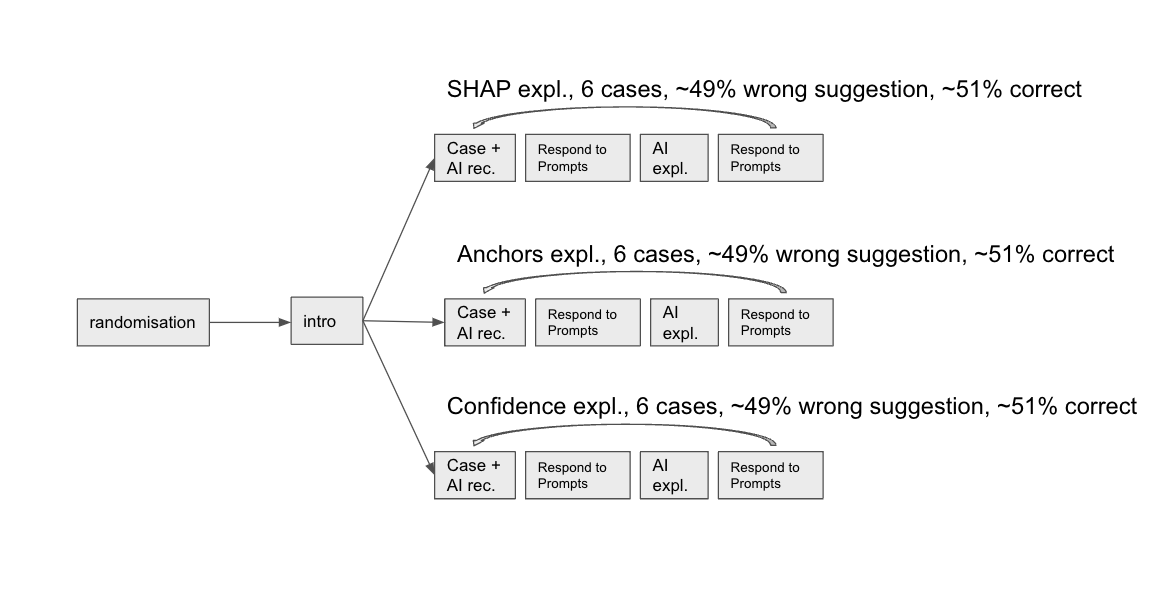
\includegraphics[width=0.8\textwidth]{figures/misleading_explanations/flowchart.png}
    \caption{Study flow}
    \label{fig:flowchart}
\end{figure*}

In both studies, each participant was shown a brief explanation of the task in question and was then asked to complete the 6 cases, with participants given a random mix of correct and incorrect cases. In each case, participants are first shown a table identifying subject of the case and an AI recommendation of what determination they should make. They are then asked to estimate the dependent variable, and rate both their confidence in the estimate and their trust in the AI recommendation on sliding scales (this is discretised to 20 points).

We code the participant's estimate as a binary $estiamte$ variable. The two sliding scale responses are coded as $confidence$ and $trust_{attitude}$ and have values between 1 and 20. As we do this in both the `before-explanation' and `after-explanation' conditions, we collect six responses from each participant in each case:  $estimate^{before}$, $confidence^{before}$, $trust_{attitude}^{before}$, $estimate^{after}$, $confidence^{before}$, and $trust_{attitude}^{after}$.  We additionally have the binary variables $answer$ and $recommendation$ indicating to true value and AI determination of the dependent variable, respectively.

In addition to these, we define $agreement^{before}$ and $agreement^{after}$ to be whether the user's estimate is in agreement with the machine's recommendation. We define $trust_{behaviour}^before$ and $trust_{behaviour}^after$ to be the extent to which the participant's confidence agrees with the machine's recommendation. Finally, in order to reason about the change in a variable due to the explanation, we define `$\Delta$' constructs for all variables with a $before$ and an $after$ case as the after-explanation value minus the before-explanation value.

More detailed definitions of all constructs can be found in Appendix \ref{app:misleadingexplanations}.

\subsection{Demographcs}

We had a total of $192$ participants complete the Salary Estimation study. These were split pseudorandomly into our three explanatory groups. By gender, $115$ were Male, $76$ were Female, and $1$ did not provide gender information. By ethnicity, $137$ were white, $10$ did not provide ethnicity, and the remaining $45$ were split among non-white ethnicities. Our participants were an average of $36.7$ years old, with the oldest being $18$ and the oldest $74$. Each applicant completed an introductory page and six cases. The average completion time for these tasks were $7$ minutes $43$ seconds, the minimum was $2$ minutes $25$, and the maximum was $36$ minutes $46$.

We had a total of $197$ participants complete the Credit Prediction study. These were similarly split into groups. By gender, $106$ were Male, $90$ were Female, and $1$ did not provide gender information. By ethnicity, $143$ were white, $11$ did not provide ethnicity, and the remaining $43$ were split among non-white ethnicities. Our participants were an average of $38.4$ years old, with the oldest being $20$ and the oldest $77$. Each applicant completed an introductory page and six cases. The average completion time for these tasks were $7$ minutes $53$ seconds, the minimum was $2$ minutes $17$, and the maximum was $30$ minutes $13$.

In both tasks, though we originally set $200$ as our target participants, some participants did not complete our task following Prolific Academic's guidelines. Data from these participants was marked incomplete and removed from consideration leaving a total of 192 and 197 participants in each study.

\subsection{SHAP and Confidence Increase Unwarranted Trust}\label{ssec:ttests}
We first test for possible increases in unwarranted trust and find that SHAP and Confidence both increase unwarranted trust on our tasks \cite{natarajan_binns_2022}. That is, when the AI recommendation is incorrect (I.e., when $answer \neq recommendation$), we find that these conditions increase trust. Furthermore, we find this result more strongly for behavioural trust than attitudinal trust in all but one test. Notably, the Anchors condition does not follow this pattern.

Table \ref{tab:delta-trust-t} shows the results of a one-sided t-test comparing $trust^{after}$ to $trust^{before}$ when $answer \neq recommendation$. A positive $t$ statistic indicates $x^{after} > x^{before}$ (I.e., $\Delta x > 0$), and a negative $t$ statistic indicates $x^{after} < x^{before}$, but, as these are one-sided tests, $p$-values will only be meaningful when $t > 0$. We show both types of trust in all three explanatory conditions on both tasks.

\begin{table*}[htbp]
    \caption{One-Sided T-Tests Comparing Trust Before- and After-Explanation}
    \begin{center}
    \begin{tabular}{ccccc}
        \toprule
        Task & Condition & Variable & t Statistic & p Value \\ 
        \midrule
        Salary Estimation & Anchors & $trust_{behaviour}$ & $0.509$ & $0.306$ \\
        & & $trust_{attitude}$ & $0.165$ & $0.434$ \\
        & SHAP & $trust_{behaviour}$ & $\mathbf{3.811}$ & $\mathbf{<0.001}$ \\
        & & $trust_{attitude}$ & $-0.886$ & $0.812$ \\
        & Confidence & $trust_{behaviour}$ & $\mathbf{2.196}$ & $\mathbf{0.015}$ \\
        & & $trust_{attitude}$ & $0.945$ & $0.173$ \\
        \midrule
        Credit Prediction & Anchors & $trust_{behaviour}$ & $1.396$ & $0.082$ \\
        & & $trust_{attitude}$ & $-2.364$ & $0.990$ \\
        & SHAP & $trust_{behaviour}$ & $1.516$ & $0.066$ \\
        & & $trust_{attitude}$ & $\mathbf{2.475}$ & $\mathbf{0.007}$ \\
        & Confidence & $trust_{behaviour}$ & $\mathbf{1.835}$ & $\mathbf{0.034}$ \\
        & & $trust_{attitude}$ & $0.940$ & $0.174$ \\
        \bottomrule
    \end{tabular}
    \label{tab:delta-trust-t}
    \end{center}
\end{table*}

Note that this is only testing for an unwarranted increase in trust, and says nothing about warranted increases or unwarranted decreases. We instrument this test as such because prior work indicates that modern explanation methods are not well-calibrated, leading us to expect such unwarranted increases \cite{miller_explainable_2023}.

\subsection{Different Explanation Styles Have Different Effects on Unwarranted Trust}\label{ssec:anovas}
We next seek to determine whether the change in trust varies between our conditions \cite{natarajan_binns_2022}. We find that such changes in trust do in fact vary between conditions. Further analysis of this variance is found in Subsections \ref{ssec:hsd-salary} and \ref{ssec:hsd-credit}.

Table \ref{tab:delta-trust-anova} contains ANOVA tests examining whether different explanation styles yielded different $\Delta trust$ values when $answer \neq recommendation$. An $F>1$ indicates that different explanation styles (I.e., SHAP, Anchors, and Confidence) have a different impact on the given trust variable, and $p<0.05$ indicates that this difference is statistically significant. However, ANOVA analyses do not indicate \emph{which} styles differ.

\begin{table}[htbp]
    \caption{ANOVAs Comparing Trust Across Explanation Styles}
    \begin{center}
    \begin{tabular}{cccc}
        \toprule
        Task & Variable & F Statistic & p Value \\
        \midrule
        Salary Estimation & $\Delta trust_{behaviour}$ & $\mathbf{3.671}$ & $\mathbf{0.026}$ \\
        & $\Delta trust_{attitude}$ & $0.925$ & $0.397$ \\
        \midrule
        Credit Prediction & $\Delta trust_{behaviour}$ & $0.066$ & $0.936$ \\
        & $\Delta trust_{attitude}$ & $\mathbf{6.213}$ & $\mathbf{0.002}$ \\
        \bottomrule
    \end{tabular}
    \label{tab:delta-trust-anova}
    \end{center}
\end{table}

In the Salary Estimation task, we find no significant results for our ANOVA $trust_{attitude}$, but do find significant results for $trust_{behaviour}$. However, in the Credit Prediction task, we find significant results for our ANOVA $trust_{attitude}$, but none for $trust_{behaviour}$. That is, in the Salary Estiamtion task, different explanations styles have a different impact on behavioural trust, and in the Credit Prediction task, different explanations styles have a different impact on attitudinal trust. We examine these two findings in Subsections \ref{ssec:hsd-salary} and \ref{ssec:hsd-credit}, respectively.

\subsubsection{SHAP Increases Behavioural Trust More than Anchors in the Salary Estimation Task}\label{ssec:hsd-salary}
We would expect that, because we found that $\Delta trust_{behaviour} > 0$ in both the SHAP and Confidence cases of the Salary Estimation Task (and in the Anchors case we did not), the means of the former two should be significantly greater than the latter. However, while we find that SHAP increases behavioural trust more than Anchors, we find no significant results relating to the Confidence condition.

Following our preregistered protocol for significant ANOVA results, we turn to Tukey's HSD as a post-hoc test \cite{natarajan_binns_2022}. Table \ref{tab:delta-trust-hsd} shows the results of this test. Note that this is again restricted to when $answer \neq recommendation$.

\begin{table}[htbp]
    \caption{Tukey's HSD Test Comparing Change in Behavioural Trust Across Explanations in Salary Estimation}
    \begin{center}
    \begin{tabular}{ccccc}
        \toprule
        Condition A & Condition B & Variable & Test Statistic & p Value \\
        \midrule
        SHAP & Anchors & $\Delta trust_{behaviour}$ & $\mathbf{2.310}$ & $\mathbf{0.022}$ \\
        Confidence & Anchors & $\Delta trust_{behaviour}$ & $0.855$ & $0.599$ \\
        SHAP & Confidence & $\Delta trust_{behaviour}$ & $1.455$ & $0.198$ \\
        \bottomrule
    \end{tabular}
    \label{tab:delta-trust-hsd}
    \end{center}
\end{table}

Table \ref{tab:delta-trust-hsd} demonstrates a significant difference in the mean of $\Delta trust_{behaviour}$ only between the SHAP and Anchors conditions when $answer \neq recommendation$. This indicates that, beyond increasing behavioural trust in incorrect AI outputs, SHAP increases behavioural trust in incorrect AI outputs \emph{more} than Anchors.

\subsubsection{SHAP and Confidence Increase Unwarranted Attitudinal Trust More than Anchors in the Credit Prediction Task}\label{ssec:hsd-credit}
We found a large negative $t$ value for $\Delta trust_{attitude}$ in the Anchors case in the Credit Prediction portion of Table \ref{tab:delta-trust-t} -- an effect that is not significant due to the one-sidedness of our tests. However, as we found only positive $t$ values for $\Delta trust_{attitude}$ in the SHAP and Confidence cases, we expect that Anchors has a negative effect on $\Delta trust_{attitude}$ relative to SHAP and Confidence. Table \ref{tab:delta-trust-anova} confirms this expectation: SHAP and Confidence both have a more positive effect on attitudinal trust than Anchors in the Credit Prediction task.

Table \ref{tab:delta-trust-anova} again follows our preregistered protocol for significant ANOVA results with a Tukey's Honestly Significant Difference (HSD) test \cite{natarajan_binns_2022}. This is again restricted to when $answer \neq recommendation$.

\begin{table}[htbp]
    \caption{Tukey's HSD Test Comparing Change in Attitudinal Trust Across Explanations in Credit Prediction}
    \begin{center}
    \begin{tabular}{ccccc}
        \toprule
        Condition A & Condition B & Variable & Test Statistic & p Value \\
        \midrule
        SHAP & Anchors & $\Delta trust_{attitude}$ & $\mathbf{1.213}$ & $\mathbf{<0.001}$ \\
        Confidence & Anchors & $\Delta trust_{attitude}$ & $\mathbf{1.030}$ & $\mathbf{<0.001}$ \\
        SHAP & Confidence & $\Delta trust_{attitude}$ & $0.183$ & $0.708$ \\
        \bottomrule
    \end{tabular}
    \label{tab:delta-trust-hsd-2}
    \end{center}
\end{table}

Table \ref{tab:delta-trust-hsd-2} shows a significant difference in the mean of $\Delta trust_{behaviour}$ between the Anchors condition and both other conditions, but no significant difference between SHAP and Confidence. This indicates that SHAP and Confidence increase unwarranted attitudinal trust relative to Anchors (although Anchors appears to actually \emph{reduce} unwarranted attitudinal trust).

Note that this does not prove that Anchors reduces attitudinal trust relative to no explanation. For this analysis, we will need another t-test. As we did not preregister this test, analysis of this phenomenon is included in exploratory analysis in Subsection \ref{ssec:anchors-decrease} \cite{natarajan_binns_2022}.

\subsection{Anchors Decrease Attitudinal Trust in a Machine}\label{ssec:anchors-decrease}
We noted already that SHAP and Confidence appear to increase trust in cases where the machine is incorrect. However, we noticed no such result for Anchors. Instead, we found that Anchors appeared to decrease end-user trust in incorrect machine outputs (I.e., when $answer \neq recommendation$). The two-sided t-test in table \ref{tab:delta-trust-t-2} confirms this.\footnote{This analysis was not preregistered.}

\begin{table*}[htbp]
    \caption{Two-Sided T-Tests Comparing Trust Before- and After-Explanation}
    \begin{center}
    \begin{tabular}{ccccc}
        \toprule
        Task & Condition & Variable & t Statistic & p Value \\ 
        \midrule
        Salary Estimation & Anchors & $trust_{behaviour}$ & $0.509$ & $0.611$ \\
        & & $trust_{attitude}$ & $0.165$ & $0.869$ \\
        \midrule
        Credit Prediction & Anchors & $trust_{behaviour}$ & $1.396$ & $0.164$ \\
        & & $trust_{attitude}$ & $\mathbf{-2.364}$ & $\mathbf{0.019}$ \\
        \bottomrule
    \end{tabular}
    \label{tab:delta-trust-t-2}
    \end{center}
\end{table*}

Table \ref{tab:delta-trust-t-2} shows that, on the two-sided t-test, we \textit{do} find that the provision of Anchors explanations decreases participant attitudinal trust in incorrect machine recommendations, at least in the Credit Prediction task. However, we do not see a similar effect on behavioural trust, and this effect is limited to only one task. 

\subsection{Behavioural and Attitudinal Trust are Highly Correlated}\label{ssec:trust-corr}
Given that many patterns observed for $trust_{behaviour}$ do not hold for $trust_{attitude}$, we might expect these variables to correlate only minimally. However, while they are mathematically distinct constructs, they are both intended to measure the same underlying phenomenon. Table \ref{tab:trust-correlation} demonstrates a high correlation between these two measurements of trust across all cases.\footnote{Though previous analyses considered only incorrect recommendations, this analysis relates \textit{all} trust, not just unwarranted trust, so we consider all cases, regardless of whether or not $answer == recommendation$.}\footnote{This analysis was only partially preregistered; we did not register this analysis in the Salary Estimation task, but we did in the Credit Prediction task \cite{natarajan_binns_2022}.}

Table \ref{tab:trust-correlation} shows a Pearson's correlation analysis across all explanatory conditions in both the before- and after- cases. We also perform this analysis on $\Delta trust_{attitude}$ and $\Delta trust_{behaviour}$.

\begin{table*}[htbp]
    \caption{Pearson's Correlation Between Attitudinal and Behavioural Trust}
    \begin{center}
    \begin{tabular}{ccccc}
        \toprule
        Task & Variable A & Variable B & Rho & p Value \\
        \midrule
        Salary Estimation & $trust_{attitude}$ & $trust_{behaviour}$ & $\mathbf{0.630}$ & $\mathbf{<0.001}$ \\
        & $\Delta trust_{attitude}$ & $\Delta trust_{behaviour}$ & $\mathbf{0.265}$ & $\mathbf{<0.001}$ \\
        \midrule
        Credit Prediction & $trust_{attitude}$ & $trust_{behaviour}$ & $\mathbf{0.612}$ & $\mathbf{<0.001}$ \\
        & $\Delta trust_{attitude}$ & $\Delta trust_{behaviour}$ & $\mathbf{0.179}$ & $\mathbf{<0.001}$ \\
        \bottomrule
    \end{tabular}
    \label{tab:trust-correlation}
    \end{center}
\end{table*}

Table \ref{tab:trust-correlation} indicates that both trust variables are highly correlated across both of our tasks. Furthermore, though the correlation between the $\Delta trust$ is more modest, it is still statistically significant.

\subsection{Anchors and SHAP Increase Participant Confidence in their Prediction}

Noting that behavioural trust is constructed from $confidence$ values, we ask: ``does providing an Anchors explanations increase participant confidence in their own decisions when the AI recommendation is incorrect?'' Table \ref{tab:delta-trust-t} supplies evidence indicating that Anchors (and SHAP) explanations increase participant confidence in their own estimations when $answer \neq recommendation$. This result agrees with \textcite{wan_explainabilitys_2022} and \textcite{bansal_does_2021}, suggesting these explanation types yield a blanket increase in participant self-confidence.\footnote{This analysis was not preregistered.}

Table \ref{tab:delta-confidence-t} contains a t-test comparing $confidence$ in all three explanatory conditions. \footnote{Note for clarity that $confidence$ is the variable indicating participant confidence in their own decisions, and `Confidence' is the condition in which the machine's explanation consists of its own confidence in its suggestion.}

\begin{table}[htbp]
    \caption{One-Sided T-Tests Comparing $confidence$ Before- and After-Explanation}
    \begin{center}
    \begin{tabular}{ccccc}
        \toprule
        Task & Condition & Variable & t Statistic & p Value \\
        \midrule
        Salary Estimation & Anchors & $confidence$ & $\mathbf{2.171}$ & $\mathbf{0.016}$ \\
        & SHAP & $confidence$ & $\mathbf{1.694}$ & $\mathbf{0.046}$ \\
        & Confidence & $confidence$ & $1.047$ & $0.296$ \\
        \midrule
        Credit Prediction & Anchors & $confidence$ & $\mathbf{1.742}$ & $\mathbf{0.042}$ \\
        & SHAP & $confidence$ & $\mathbf{3.473}$ & $\mathbf{<0.001}$ \\
        & Confidence & $confidence$ & $0.752$ & $0.226$ \\
        \bottomrule
    \end{tabular}
    \label{tab:delta-confidence-t}
    \end{center}
\end{table}

Table \ref{tab:delta-trust-t} demonstrates that, while Confidence shows no significant effects on either task, participants shown an Anchors or SHAP explanation grow significantly more confident in their prediction, indicating that providing an Anchors or SHAP explanation serves to increase a participant's confidence in their \emph{own estimate}.

\subsection{Explanations Impact Trust Differently When the Machine is Correct}
Note that properly calibrated trust would involve both distrusting the machine when it is wrong and trusting it when it is right. To assess the latter, we give a brief evaluation of what happens in the cases where the AI is correct, I.e. where $answer == recommendation$. Table \ref{tab:delta-trust-t-positives} contains the results of these analyses.\footnote{These analyses were not preregistered.}

\begin{table*}[htbp]
    \caption{Two-Sided T-Tests Comparing Trust Before- and After-Explanation when $answer == recommendation$}
    \begin{center}
    \begin{tabular}{ccccc}
        \toprule
        Task & Condition & Variable & F Statistic & p Value \\ 
        \midrule
        Salary Estimation & Anchors & $trust_{behaviour}$ & $0.502$ & $0.616$ \\
        & & $trust_{attitude}$ & $\mathbf{-2.337}$ & $\mathbf{0.020}$ \\
        & SHAP & $trust_{behaviour}$ & $0.295$ & $0.768$ \\
        & & $trust_{attitude}$ & $-1.385$ & $0.168$ \\
        & Confidence & $trust_{behaviour}$ & $\mathbf{2.410}$ & $\mathbf{0.017}$ \\
        & & $trust_{attitude}$ & $\mathbf{3.254}$ & $\mathbf{0.001}$ \\
        \midrule
        Credit Prediction & Anchors & $trust_{behaviour}$ & $\mathbf{3.013}$ & $\mathbf{0.003}$ \\
        & & $trust_{attitude}$ & $\mathbf{-2.487}$ & $\mathbf{0.014}$ \\
        & SHAP & $trust_{behaviour}$ & $0.207$ & $0.836$ \\
        & & $trust_{attitude}$ & $\mathbf{3.538}$ & $\mathbf{0.001}$ \\
        & Confidence & $trust_{behaviour}$ & $\mathbf{2.863}$ & $\mathbf{0.005}$ \\
        & & $trust_{attitude}$ & $\mathbf{2.461}$ & $\mathbf{0.015}$ \\
        \bottomrule
    \end{tabular}
    \label{tab:delta-trust-t-positives}
    \end{center}
\end{table*}

\subsubsection{Confidence Explanations Increase Warranted Trust}
Positive $\Delta trust$ values in all cases in table \ref{tab:delta-trust-t-positives} demonstrate that Confidence explanations increased both measured types of user trust in the AI output when the model is correct across both tasks.

\subsubsection{Anchors Explanations Decrease Warranted Attitudinal Trust}
Table \ref{tab:delta-trust-t-positives} also demonstrates that providing Anchors explanations yields a \emph{decrease} in $trust_{attitude}$. This, alongside the finding from Subsection \ref{ssec:anchors-decrease}, indicates that Anchors explanations have a negative impact on $trust_{attitude}$, regardless of model correctness.

\subsubsection{SHAP Explanations Increase Warranted Attitudinal Trust in the Credit Prediction Task}
SHAP explanations increase Warranted attitudinal trust in the Credit Prediction Task as shown in table \ref{tab:delta-trust-t-positives}. However, the effect is not mirrored in tests of $trust_{behaviour}$ or on the Salary Estimation Task.

\subsection{Limitations}

\subsubsection{Generalisation and External Validity}
The external validity of our results may be challenged due to our use of artificial tasks and benchmark datasets. Indeed, field studies with decision-makers in real deployments would be needed to yield results that apply uncontroversially in a given domain. Along a similar vein, one might contend that the use of only two tasks is insufficient to generalise our results to other domains. One might also challenge external validity of our results due to our limited selection of only three explanatory conditions (only two of which are commonly used xAI methods).

We choose two similar datasets in a narrow domain (human-in-the-loop binary classification tasks with definite but non-obvious ground truth) as we do not wish to confuse our primary research questions with questions surrounding generalisation. Similarly, we contend research on further tasks is extraneous to the primary questions. More information on our specific selection of cases can be found in Appendix \ref{app:misleadingexplanations}.

We choose SHAP and Anchors as popular candidate explanations from different styles, as we wish to demonstrate conditions under which unwarranted trust may and may not arise. We choose Confidence as a third condition as this condition acts as a sort of baseline. More information on our choice of explanation algorithms can be found in Appendix \ref{app:misleadingexplanations}.

That said, insofar as performance on benchmark datasets can be expected to generalise, we believe our findings will extend to predictive tasks whose answers are difficult enough to both human and AI systems and where performance is distributed differently between them. We do not expect our findings to generalise to tasks where the answers are either immediately evident to the user (such as predicting whether a given image contains a cat) or so difficult as to be impossible to the naked eye (such as gene function prediction). And while we do expect our findings to generalise beyond tabulated binary classification tasks, said generalisation does not impact the primary significance of these findings: xAI developers, evaluators, and implementers alike should concern themselves with the possibility of unwarranted trust.

\subsubsection{Effect on Overall Task Performance}

We have focused exclusively on the phenomenon of misplaced trust when the AI output is incorrect. However, while problematic, this has to be weighed against the effect an xAI method has on overall task performance. It might be remarked that, even if SHAP explanations increased misplaced trust, if they increased performance on the task overall, that would still be desirable. Indeed, relative to no explanation at all, SHAP may be beneficial simply because of its effect of increasing user trust overall. (The effect of an overall increase in trust in AI outputs will depend on the relative accuracies of the AI and the human.)

However, we do not contend that the unwarranted trust issue renders SHAP explanations useless. We instead contend that they may lead to dangerous abuse. When implementing xAI algorithms in human-in-the-loop tasks, implementers should consider the possible harms of this potential for abuse, especially when these tasks have definite but unobvious ground truth. Furthermore, those developing xAI applications for use in these contexts should strive to develop explanation methods that appropriately calibrate trust in addition to increasing overall task performance.

\subsection{Discussion}
In this chapter, we investigate the extent to which three different AI explanation methods can create unwarranted trust in their underlying AI systems on a specific set of tasks. Specifically, we look at whether any of our Anchors, SHAP, or Confidence explanatory conditions increase trust in a model when that model is wrong. We restrict our analysis specifically to the subset of tasks human-in-the-loop where the ground truth of the prediction is neither subjective nor immediately evident to the human. We perform analyses on two tabular binary prediction tasks that satisfy this condition: Salary Estimation and Credit Prediction.

We conclude here that SHAP and Confidence explanations are liable to induce unwarranted trust under these circumstances, but we find no evidence of the same for Anchors. This demonstrates that, in these cases, neither SHAP nor Confidence serve to correctly calibrate trust in AI outputs. Rather, they blindly increase trust in these outputs, encouraging users to incorrectly agree with the AI explained. Furthermore, we find that, while Anchors may not induce unwarranted trust, it instead fosters blanket distrust for the AI and increased confidence in user decision-making. As such, the effect of Anchors explanations on trust calibration may not be positive overall; it is dependent on the distribution of correct vs. incorrect disagreements between user and AI. (Indeed, for certain distributions of correct vs. incorrect disagreements, all three explanation styles may have a negative overall effect on trust calibration.) These findings suggest that, at least under the conditions outlined, xAI may be at best useless and at worst actively harmful in its effects on human trust calibration. 

Though trust is often a component of both design and evaluation, \emph{trustworthiness} is often overlooked \cite{jacovi_formalizing_2021,lundberg_unified_2017,ribeiro_why_2016,jacobs_how_2021}. It is often assumed that these explanations draw directly from model outputs, and are therefore akin to oracles that grant a general understanding of the system. In \textcite{natarajan_trust_2023}, we argue for a paradigm shift against this use of explainable AI systems, and instead argue that systems should be developed, evaluated, and used for specific purposes. We agree with this sentiment. In fact, we contend it is not itself problematic that user trust in AI systems might increase as a result of xAI. But it is problematic that user trust in wrong decisions made by AI systems may increase in response to the use of a maximally trust-inducing explanation method. Particularly in human-in-the-loop tasks with definite but unclear ground truth, trust should not be considered the \emph{raison d'etre} of xAI. More heed should be instead paid to \emph{calibrating} trust in AI systems and to ensuring that explanations are sufficiently well-calibrated for the use cases they are considered for.

\section{Conclusion}
% Clearly, post-hoc and intrinsically interpretable are very different. We clearly need to study them separately. That's what the next two chapters do
% \begin{savequote}[8cm]
% Alles Gescheite ist schon gedacht worden.\\
% Man muss nur versuchen, es noch einmal zu denken.

% All intelligent thoughts have already been thought;\\
% what is necessary is only to try to think them again.
%   \qauthor{--- Johann Wolfgang von Goethe \cite{von_goethe_wilhelm_1829}}
% \end{savequote}

\chapter{\label{ch:usingxai}Using Post-Hoc Explainable AI to Identify Talent: Explaining an Applicant Scoring Algorithm with Shapley Values}

% Notes
% Can we replicate misleading explanations? We have data from this year and last.
% Are there classes of cases which are plausibly connected to the types of areas that the old non-SHAP decision-making process would have yielded? Can we independently identify these in the new cohort?
% Maybe: does the new “SHAP” process reduce surprise/disagreement with the algorithm
% Can we do something qualitatively?
% How does SHAP have the right kind of effect on decision-making
% Could we measure the magnitude of disagreement between humans and algorithms?
% Then qualitatively, ask people why they disagreed with algorithm scores?
% It’s hard to tie this stuff specifically to the under/over-reliance stuff unless we can argue that more disagreement is good
% We don’t have ground truth, so the misleading stuff is difficult, but we can argue that disagreement/engagement are both good. We can qualitatively compare the richness/level of understanding/ perceived helpfulness.
% Do they have more reasons for disagreeing? More specific reasons?
% Fundamental thought: if SHAP helps the decision makers understand the reason why, but we don’t care about that factor, wouldn’t it be better to change the model so as to not consider that factor as much? Maybe explanation tools are a way of modifying the model here? Can the case study / utility be a change to the model? Maybe decision-makers need to be in the middle of their decision-making process to reconsider the principles, and maybe these decisions are best made using SHAP?
% Alternative case study idea: maybe various reviewers meet and extract generalisations from the SHAP charts they’ve been using?
% The idea of individual justice: no set of criteria exists that correctly applies to every case; under this principle, the value of SHAP is to say that “this particular case is an exception to the model, since you don’t want to mess with it in general, you just want to make an exception in this case”
% The underlying model is trying to predict accept/reject based on previous candidates, which is sort of a ground truth, but not the only truth that decision-makers are interested in; this is a major difference from the misleading explanations thing
% Another major difference: decision-makers have access to a lot of information the model doesn’t; part of the role of SHAP is to tell decision-makers when that info is important
% It sounds like the evaluation is qualitative / not-based-on-ground-truth. It’s instead based on decision-maker feedback about when they rely on the explainer system
% More satisfying to have some case study
% Can I collect with/without SHAP information on how they collect decisions?
% Could we apply SHAP to previously made decisions and use SHAP to elucidate the past year confusions? This was a part of the design process
% Does this necessarily need to be qualitative?
% Also: do we want to change the model next year based on the decisions made with this algorithm? I.e., should we rely more or less on specific features? This is sort of necessarily qualitative. Also, this could be taken from the design process, since this happened in the interviews
% This makes a good argument for why we can’t just do an RCT 

\minitoc

\section{Introduction}
We develop a SHAP-based procedure for explaining the decisions made by an applicant scoring algorithm used in a talent investment organisation. We take into account the original functions of SHAP explanations and provide a contract for the intended use case of our procedure: to systematically reveal insights about the underlying algorithm itself, help us better understand counterintuitive results, and instruct us on where this algorithm should be modified. We explore decisions made by the talent investment organisation and analyse the applicant scoring algorithm using the SHAP tool. We discover that professionals prefer a mixture of verbal and visual explanation, and often require context for decisions not in a real selection procedure, as a case study. Finally, we discuss the potential for extending this tool to use in decision-making and note strategies to combat mis-calibrated trust.

(To-do)

\section{....}

(To-do)

% \begin{savequote}[8cm]
% Alles Gescheite ist schon gedacht worden.\\
% Man muss nur versuchen, es noch einmal zu denken.

% All intelligent thoughts have already been thought;\\
% what is necessary is only to try to think them again.
%   \qauthor{--- Johann Wolfgang von Goethe \cite{von_goethe_wilhelm_1829}}
% \end{savequote}

\chapter{\label{ch:iaicasestudy}A Human-Centric Approach to Identifying Talent With Intrinsically Interpretable Models [WIP]} % Maybe this is two chapters? The co-design could be one chapter, and the SPF itself could be another?

\minitoc

\section{Introduction}
(To-do)

\section{Background}
(To-do)

% \subsection{Dviersity as an institutional value}
% conservative critiques as `too diverse' david goodhart

% combahee river collective `identity politics' `The term “identity politics” was first popularized by the 1977 manifesto of the Combahee River Collective, an organization of black feminist activists.'
% intersectionality (pre-crenshaw?)
% standpoint epistemology
% zetetic 
% `Reasons to think the oppressed have such an advantage include that they tend to have: more informative experiences of oppression (e.g. Mills 1998), greater incentives to learn about and criticize oppression (e.g. Jaggar 1983), and access to networks of other oppressed people who are themselves epistemically advantaged with respect to oppression (e.g. Dror 2023).' tuckwell and yeo

% wheel of academic privilege example

% neoliberal multiculturalism produces racialised distinctions of `good diversity' (a racially diverse football team) and `bad diversity' (racialised subjects criticising foreign policy are seen as `failing to integrate') - lentin and titley 2011

% ` diversity is a malleable discourse suffused through
% a variety of institutional practices and political frameworks. Diversity may be a
% hybrid product of strands of contemporary thinking on identity, difference, power
% and social justice, but this does not entail that discourses and practices of diversity
% offer the enabling or subversive possibilities associated with it in all or even many
% contexts.' lentin and titley - benneton

% the diversity bargain - warikoo

% \subsection{Diversity Concepts and Measures}
% draw significantly from Steel et al

% in science

% budescu
% steel et al
% schumann
% entrofy - huppenkothen et al

% \subsection{Employee diversity for productivity}
% page et al the diversity bonus, the difference
% ostergaard

% \subsection{Fair ML}
% Group fairness
% Individual fairness - binns, fleisher

% \subsection{Critiques of Diversity}
% Taiwo and Rossi
% Ahmed:
% on being included: `commitment to diversity is frequently substituted for a commitment to actual change'
% documenting rather than doing

% diversity training - not clear if it works `We suggest that the enthusiasm for, and monetary investment in, diversity training has outpaced the available evidence that such programs are effective in achieving their goals.' devine et al

\section{Methods Part 1}
\subsection{Researcher Bias}
Following the methodology of \textcite{braun_using_2006}, we acknowledge that our own biases may (positively or negatively) influence our research. We are a team of three researchers: one South Asian man from the US, one South Asian woman from India, and one white man from the UK.

\subsection{Our Study}
Our study is broken into two components: a series of interviews with talent identification professionals and two participatory design workshops with said professionals. In the first session, we seek to ascertain how these professionals understand diversity, how they operationalise it in their work, and how they envision using technology to assist them in that process. In the second session, we show these professionals a series of mock-up designs drawn in response to the interviews, then we aim to collaboratively design tools that can help them better operationalise diversity.

\subsection{Interviews and Thematic Analysis}
Our interviews aim to answer three research questions:

\begin{enumerate}
    \item What is diversity?
    \item Which elements of diversity matter in a talent identification context? Why?
    \item How would you envision technology assisting you in operationalising diversity?
\end{enumerate}

In answering our first set of research questions, we follow \cite{braun_using_2006}'s methodology for thematic analysis. We first conduct 45-minute semi-structured interviews with 15 talent identification professionals. In each interview, we first ask general questions about their selection methodology; we next ask specifically about diversity and it's role in selection; we move on to a ``crazy 8s'' exercise designed for participatory design; we conclude with a ``magic app'' exercise, also designed for participatory design. A question-by-question protocol for these interviews is found in Appendix \ref{app:protocolmockup}. However, following the methodology of \cite{braun_using_2006}, we do not limit our analysis to these questions. Instead, we deviate from this script as guided by the conversations and our overarching research questions, then we allow themes to emerge naturally from the data.

After interviewing participants, the interviewer transcribes the interviews and anonymizes them. Two researchers then independently ``open-code'' each anonymized transcript, looking for anything relevant to our research questions. The researchers meet to discuss their open codes, and collaborate in the process of clustering these codes into subthemes and themes.

\subsection{Design Workshops}
Before this workshop, we use the findings from the thematic analysis to design a series of mock-up technologies. Our research question for this workshop is, for each mock-up: ``How can this mock-up help you better promote diversity in talent identification?''. A full protocol for this workshop is found in Appendix \ref{app:protocolmockup}.

After running this workshop, the researchers use written notes and meeting recordings to draw conclusions about the relative utility of each mock-up, and extract guidelines for the design of future tools.

\section{Results Part 1}
% \begin{center}
%     \label{tab:allthemes}
%     \begin{tabular}{| l | l | l | l | l | l |} 
%         \textbf{Why Diversity} & \textbf{Types of Diversity} & \textbf{Operational Risks and Considerations} & \textbf{Fairness and Bias} & \textbf{Scholarship Goals} & \textbf{Merit}\\
%         Different perspectives & Socioeconomic & Outreach & Fairness & Impact & Performance relative to disadvantage\\
%         \emph{...In the same room} & \emph{Parental income} & Support & \emph{...to all applicants} & \emph{...on all applicants} & Measurement\\
%         Representativeness & \emph{Parental education} & \emph{...during the application process} & \emph{...to the selected scholars} & \emph{...on the selected scholars' performance} & Merit vs. diversity\\
%         \emph{...of a general population} & \emph{Generational wealth} & \emph{...after selection} & \emph{...to the scholarship} & \emph{...on the selected scholars' opportunities} & \\
%         \emph{...of the eligible population} & Sex, gender, and sexuality & Selectors & Bias & \emph{...by the selected scholars on the world} & \\
%         \emph{...of the applicant population} & \emph{Sex} & Applicant fraud & \emph{Measurement bias} &  & \\
%         \emph{...of a taget population } & \emph{Gender identity} &  & \emph{Decision-makers' bias (prejudicial)} &  & \\
%         Boosting disadvantaged groups & \emph{Sexual orientation} &  & \emph{Decision-makers' unique perspective (probative)} &  & \\
%          & Geography &  & Transparency &  & \\
%          & \emph{Nationality} &  & \emph{Transparency as fairness} &  & \\
%          & \emph{Global south} &  & \emph{...during the application process} &  & \\
%          & \emph{Region} &  & \emph{...after selection} &  & \\
%          & Types of thinking &  &  &  & \\
%          & \emph{Subject area interest} &  &  &  & \\
%          & \emph{Personality type} &  &  &  & \\
%          & \emph{Core beliefs} &  &  &  & \\
%          & \emph{Problem solving approaches} &  &  &  & \\
%          & \emph{Political views} &  &  &  & \\
%          & Race &  &  &  & \\
%          & \emph{International categorisations of race} &  &  &  & \\
%     \end{tabular}
% \end{center}


\subsection{Participants}
We interview talent identification professionals (N=15) from two talent investment programs. These professionals provided information on their roles in the selection process, and optionally provided demographic information; this information is shown in Tables \ref{tab:roles} and \ref{tab:demo}.

\begin{center}
    \label{tab:roles}
\end{center}

\begin{center}
    \label{tab:demo}
\end{center}


\subsection{Why Diversity}
A central theme of our investigation was the question of why diversity matters. To this end, we asked questions like ``What is diversity?'' and ``Why does diversity matter?''. We found that answers to these questions were closely related, and were able to cluster answers to these questions into three central subthemes: `different perspectives', `representativeness', and `boosting disadvantaged groups'. These are listed as subthemes of `Why Diversity' in Table \ref{tab:whydiv}.

\begin{table}[h]
    \centering
    \caption{Themes and Subthemes Related to What Diversity is and Why Diversity Matters}
    \label{tab:whydiv}
    \begin{tabular}{|l|} 
        \hline
        \textbf{Why Diversity} \\
        \hline
        Different perspectives \\
        \emph{...In the same room} \\
        Representativeness \\
        \emph{...of a general population} \\
        \emph{...of the eligible population} \\
        \emph{...of the applicant population} \\
        \emph{...of a taget population } \\
        Boosting disadvantaged groups \\
        \hline
    \end{tabular}
\end{table}

\subsubsection{Different Perspectives}
The first subtheme we identified was `different perspectives'. Participants frequently mentioned that diversity was important because it brought different perspectives into the same room. This was seen as important for a few related reasons, e.g., the ability to see problems from different angles and the ability to make better decisions. Several participants referred to the: ``benefits of diverse perspectives''. One wrote, when discussing their personal experience working with winners in a talent investment program, that there is: ``magic happening with lots of...diverse perspectives in the room''. Peoples' experiences were particularly relevant here. As one participant writes: ``you want to have diverse perspectives from people who look different with different experiences''.

\subsubsection{Representativeness}
The second subtheme we identified was `representativeness'. This, we observed, was often spoken of in relationship to a larger population. Most frequently, participants spoke of the importance of having a cohort that was representative of the `eligible population'. I.e., one participant said: ``[You want] a community which is representative of where you are selecting young people from''. Others spoke of this in broader, more general terms: ``you have that...broad...representation of people''. Participants identified the importance of building a cohort that variously: ``reflects the diversity of the countries'' and is ``more representative of the national population than the STEM field already is'' (the latter participant was speaking specifically of selecting STEM applicants).Others talk about representation of a particular target population, i.e.: ``representation...because that gives you insight for the people that you're trying to serve,'' and ``you have to be....reflective of your market''. Finally, selectors discussed the importance of representing an applicant population: ``[We want] a cohort that is representative of the pool''.

\subsubsection{Boosting Disadvantaged Groups}
The final subtheme we identified was `boosting disadvantaged groups'. This was often spoken of in individual terms, speaking of particular applicants in need of support. I.e.: ``identify those talents and specifically boost up people who are in need of support''. One participant identified `boosting' as a key metric for the programme: ``we need to know that...we have some level of...impact here, and...if all we're doing is supporting someone who is already on an amazing trajectory and then maybe that means we're not altering their trajectory at all. That's a question of efficiency of our dollars.''

However, this individualistic metric for success was often also identified with underrepresented or disadvantaged groups. One participant said: ``The focus on gender has been to give the sex that has had the least opportunity the opportunity in this program.''

\subsubsection{Relationships Between Subthemes}
Many selectors identified the word `diversity' with the `representativeness' subtheme. For example, one said: ``if you're doing scholarship programmes, the world is diverse. So if you want to do a global programme, then you have to be diverse''. Nonetheless, these selectors also variously identified our other subthemes as reasons diversity is important. The same selector said: ``The purpose of diversity on the gender aspect was to make sure that biological male female were getting equal opportunities''.

\subsection{Types of Diversity}
Another central focus of our investigation was on different types of diversity. We asked participants to break down their understanding of diversity into different elements, and to discuss why these elements were important. We found that participants identified a wide range of different types of diversity, which we clustered into a series of subthemes. These subthemes are listed as subthemes of `Types of Diversity' in Table \ref{tab:typesdiv}.

\begin{table}[h]
    \centering
    \caption{Themes and Subthemes Related to Types of Diversity}
    \label{tab:typesdiv}
    \begin{tabular}{|l|}
        \hline
        \textbf{Types of Diversity} \\
        \hline
        Socioeconomic \\
        \emph{Parental income} \\
        \emph{Parental education} \\
        \emph{Generational wealth} \\
        Sex, gender, and sexuality \\
        \emph{Sex} \\
        \emph{Gender identity} \\
        \emph{Sexual orientation} \\
        Geography \\
        \emph{Nationality} \\
        \emph{Global south} \\
        \emph{Region} \\
        Race \\
        \emph{International categorisations of race} \\
        Types of thinking \\
        \emph{Subject area interest} \\
        \emph{Personality type} \\
        \emph{Core beliefs} \\
        \emph{Problem solving approaches} \\
        \emph{Political views} \\
        \hline
    \end{tabular}
\end{table}


Notably, in addition to the standard demographic categories commonly considered `demographic diversity', participants identified a wide range of other types of diversity commonly termed `cognitive diversity' \cite{page2019diversity}. These included `subject areas of interest', `personality type', `core beliefs', `problem solving approaches', and `political views'.

\subsubsection{Socioeconomic}
Participants frequently identified socioeconomic diversity as particularly important in the context of a talent investment program. Indeed, one participants said: ``Socioeconomic [diversity] is probably the most important''. Another say: ``Socioeconomic background is like number one from my perspective''. This was identified as particularly important for several reasons. Participants stated: ``Because right now the SAT, for example, is more highly correlated to socioeconomic status than it is to anything else'', and: ``It's a scholarship scheme, so I think it should be for kids who cannot afford normally the fees at the university''.

Outside of the standard categorisations by income and wealth, participants also identified ``familial education level'' or ``family education backgrounds'' as a particularly important metric for understanding socioeconomic diversity in a scholarship context. One participant noted that socioeconomic status varied in both meaning and measurement from country to country: ``For example, in Columbia, there's a whole society to organise on a 1 to 7 scale for socioeconomic status''.

\subsubsection{Sex, gender, and sexuality}
While all participants noted some manner of sex, gender, and sexuality diversity as important, participants disagreed on the relative emphasis that should be place on each. One participant noted: ``[Sex] is important. I think it will get diluted if we focus on identity gender because....the purpose of diversity on the gender aspect was to make sure that [men and women] were getting equal opportunities''. Another noted that, while sexual identification diversity was important in other contexts, they ``wouldn't select for that'' in this context. Others listed ``Sexual orientation'' and ``Gender'' as important metrics for understanding diversity in a scholarship context. However, save for the participant who noted the distinction between sex and identity gender, participants expressed reluctance to discuss the relationships between this difficult concepts.

\subsubsection{Geography}
Participants frequently mentioned the importance of ``[A] wide array of different geographical [representation]''. Others mentioned a ``Regional distribution'' alongside the geographic one.

In particular, emphasis was placed on geographic markers of socioeconomic status such as  the ``Global South'', ``Indigenous communities'', and ``Low income countr[ies]''. One participant noted: ``Immigration status is tied so closely to socioeconomic status'', while another noted that ``[Geography] is connected to socioeconomics because we know there are some poorer country and rich countries''. Others still asked questions like ``Do they have a passport?'' and ``Are they in a refugee camp?''.

Furthermore, participants saw it as important that their programmes had ``Global reach''. They expressed a desire for: ``Diversity of people coming from variety of places''.

\subsubsection{Race}
While many participants identified race as an important dimension of diversity, none suggested we explicitly select for racial diversity. Several participants instead noted the difficulty of measuring race in a global context: ``Racial categories obviously vary by country''. One participant noted: ``[In places] like Brazil or England, there's a different categories of race than there are in the US...[In Brazil] there's a board of people who decide what people's race are''. In a global context, however, many participants pointed to relationships between geography and race, and hence suggested diversifying across geography in place or race: ``If it's an international programme then you can use geography as a proxy''.

\subsubsection{Types of Thinking}
One participant noted that: ``You want as much representation from different different types of thinking as you can, because I want perspectives to be listened to equally''. This manifested in many ways.

Participants tended to express the belief that personality-type-diversity could improve group cohesion: ``With that is understanding personality types be able to tell which two like which people would get on well with each other.'' One participant suggested a ``Personality test'', and another specifically mentioned a desire to diversify across ``Openness''.

However, while personality type was seen as important, core beliefs were seen as even more so. One participant noted and interest in diversity of ``Interests politically''. Another expressed a desire for diversity of ``peoples core beliefs are that's separate from religion'', and also noted: ``I would try to have a good representation of....religious groups''.

\subsection{Operational Risks and Considerations}
While our study did not focus on the operational aspects of selection, several selectors' understanding of diversity was closely tied to the operational realities of selecting for and running a scholarship. In answering our questions, several participants identified operational risks or considerations that impacted their understanding of diversity. These are listed as subthemes of `Operational Risks and Considerations' in Table \ref{tab:operational}.

\begin{table}[h]
    \centering
    \caption{Themes and Subthemes Related to Operational Risks and Considerations}
    \label{tab:operational}
    \begin{tabular}{|l|}
        \hline
        \textbf{Operational Risks and Considerations} \\
        \hline
        Outreach \\
        Support \\
        \emph{...during the application process} \\
        \emph{...after selection} \\
        Selectors \\
        Applicant fraud \\
        \hline
    \end{tabular}
\end{table}

\subsubsection{Outreach}
While our study was focused primarily on selecting a diverse cohort from a fixed applicant pool, several participants immediately began answering questions from the perspective of outreach with the goal of growing a more diverse pool of applicants to select from. In particular, participants suggested that ``Using technology for....targeted outreach'' could help improve overall cohort diversity before selection even begins. One said: ``Giving you very clear signposting on where you may want to focus, you know further recruitment or outreach or whatever it might be to make sure that your programme is diverse at the end of the day''. Another added: ``You can target your outreach dollars to communities where you know that underrepresented talent exists''.

\subsubsection{Support}
Similarly, participants suggested that technology could enable the support of applicants from underrepresented groups, which would also improve diversity. One participant suggested that technology could be used to provide: ``[Support] to keep people that you're attracting from underrepresented backgrounds and help them get across the the finish line''. While others focused on the: ``Support [applicants] need to actually get through your programme'', i.e., supporting applicants after acceptance. Another suggested that technology could be used to provide support to applicants ``after selection''.

\subsubsection{Selectors}
Other applicants noted that diversity did not apply merely to applicants. Instead, for programs where large groups of selectors assist in the selection process, ``Tracking the diversity of of the selectors'' and ``[Monitoring] how their scoring and reviewing applicants [for] prejudice or biases''.

\subsubsection{Applicant fraud}
Finally, a persistent concern with selecting based on particular diversity characteristics, especially self-reported metrics of diversity characteristics, was the potential for applicant fraud. One participant requested: ``A fraud detector'', while another expressed a desire to ensure that the process ``Isn't super gameable''.

\subsection{Fairness and Bias}
Though not a type of diversity as we have understood it here, many applicants referenced similarities between diversity metrics and metrics of fairness or bias. Furthermore, several suggested that improving fairness while reducing bias would likely yield a more diverse cohort. These themes are reflected in Table \ref{tab:fairnessbias}.

\begin{table}[h]
    \centering
    \caption{Themes and Subthemes Related to Fairness and Bias}
    \label{tab:fairnessbias}
    \begin{tabular}{|l|}
        \hline
        \textbf{Fairness and Bias} \\
        \hline
        Fairness \\
        \emph{...to the applicants} \\
        \emph{...to the world} \\
        Bias \\
        \emph{Measurement bias} \\
        \emph{Decision-makers' bias (prejudicial)} \\
        \emph{Decision-makers' unique perspective (probative)} \\
        \hline
    \end{tabular}
\end{table}

\subsubsection{Fairness}
Participants discussed that it was important that applicants: ``Get fair chance on their on their academic merit''. This translated to an emphasis on ``Fairness in the assessment''.

However, participants also noted that ``The way the world works is unfair'', and found it important that the programme is: ``Making sure that the world is fairer by bringing more diversity to this world''. In this way, participants found: ``[The] representative thing....goes back to fairness''. One participant noted that: ``Affirmative action....can come across as unfair to some people, but....it's trying to balance things out when things have been so unequal for so long''.

\subsubsection{Bias}
Participants also discussed bias as both a human- and machin-decision-making problem. Many participants appealed to technology's ability to be comparatively impartial as an important mitigator of bias, I.e., one participant repeatedly requested a: ``Non-biased program''; another stated a preference for: ``'ata analysis to make decisions on who we should be supporting as opposed to having humans try to make those decisions with all their biases''. However, others noted that common machine decision-making paradigms amplify bias, and that it was important to be aware of this: ``AI has a lot of bias in it''.

Others noted the possibility for technology to elucidate biases in both humans and machines. One participant requested: ``Some kind of tool that can detect bias in a selection''.

\subsection{Programme Goals}
Talent identification professionals from both programmes identified a series of goals for their programmes. These goals were discussed by both groups as an intended form of ``impact'' and both groups closely related achieving their goals to their answers to why diversity mattered. As these programmes wish to remain anonymous, we refrain from detailing their goals themselves, but we include this theme for reference in Table \ref{tab:scholarshipgoals}.

\begin{table}[h]
    \centering
    \caption{Themes and Subthemes Related to Programme Goals}
    \label{tab:scholarshipgoals}
    \begin{tabular}{|l|}
        \hline
        \textbf{Scholarship Goals} \\
        \hline
        Impact \\
        \emph{...on all applicants} \\
        \emph{...on the selected scholars' performance} \\
        \emph{...on the selected scholars' opportunities} \\
        \emph{...by the selected scholars on the world} \\
        \hline
    \end{tabular}
\end{table}

\subsubsection{Impact}
Participants found key goals of their program to include: ``Orient[ing] [scholars] towards social impact or using their talent for good''. They tended to encourage: ``[Scholars'] working towards something impactful over the course of their career''.

\subsection{Merit}
Finally, many participants reflected on the relationship between merit and diversity. While some participants saw these as competing goals, others saw them as complementary. In particular, complementary views often viewed merit as a form of performance relative to specific advantages, or noted that many of our measurement tools are biased across our chosen diversity dimensions. These themes are reflected in Table \ref{tab:merit}.

\begin{table}[h]
    \centering
    \caption{Themes and Subthemes Related to Merit}
    \label{tab:merit}
    \begin{tabular}{|l|}
        \hline
        \textbf{Merit} \\
        \hline
        Performance relative to disadvantage \\
        Measurement \\
        Performance vs. diversity \\
        \hline
    \end{tabular}
\end{table}

\subsubsection{Performance relative to disadvantage}
Many participants identified merit as something difficult to disentangle from performance. One participant noted that applicants may appear less qualified because they: ``Didn't have the chance; didn't have the opportunities'', while others with the opportunities will appear more qualified. Another participant began by asking: ``How good is their 3A stars based on where they've come from?'', then proceeded to reflect that ``Your performance relative to your opportunity or maybe expected performance'' is a key indicator of merit.

\subsubsection{Measurement}
Closely related, participants questioned our ability to measure merit independent of opportunity: ``[Whether they perform well] because they have the opportunity or because they are brilliant – I think that these two are really difficult to untangle.'' Another noted that ``Contextual factors mess up our otherwise seemingly objective measures of merit....national context and family income is messing up your ability to measure the thing you actually care about''. They continued to note that they: ``Need to pay attention to [diversity] because it's messing up your measures of what you actually care about''.

\subsubsection{Performance vs. diversity}
Finally, participants noted occasions where performance and diversity were ostensibly competing goals. However, even here, participants recognised that observed performance and actual merit may differ. One participant noted that: ``Overriding aim is for [the programme] to be as diverse as is possible but still meet a standard....relative score of like how good their application is based on all these kind of contextual factors''. Another requested a technology that helps discover how: ``Close you are to your idealised diversity targets and how close you are to maximising whatever it is you think your your you're maximising in your in your performance scores''.

\section{Methods (Part 2)}
\subsection{Design Mock-ups}
We apply the results of our thematic analysis to design a series of mock-up technologies. These technologies help talent identification professionals better understand and operationalise diversity in their selection processes. We then present these mock-ups to participants in participatory design workshops. As the participants all come from two separate talent investment programs, we present run one workshop for each group. Furthermore, before presenting to the broad audience of each group, we run two `pilot' workshops, where we tweak the mock-ups based on feedback from a small group of participants. Thus, while the prototypes are broadly similar between the two groups, minor differences occur between prototypes shown to each group. These prototypes are shown in Appendix \ref{app:protocolmockup}.

In particular, while we sought to draw a distinction between ``representativeness'' and ``entropy'' measurements of diversity in Figures \ref{fig:representativeness} and \ref{fig:entropy} (based on the ``Representativeness'' and the ``Different perspectives'' themes, respectively), one talent investment organisation requested that we elide that distinction so as to better fit with their current selection process. Thus, though we have three cohort-level-mockups, we present Figures \ref{fig:representativeness} and \ref{fig:entropy} to one group, and we present Figure \ref{fig:diversity} to the other. We present all three of Figures \ref{fig:demographic}, \ref{fig:impact}, and \ref{fig:advantage} to both groups. (Note here that Figures \ref{fig:demographic} and \ref{fig:impact} are based on the ``Representativeness'' theme, while Figure \ref{fig:advantage} is based on the ``Boosting disadvantaged groups'' theme.)

\subsection{Design Workshops}
Our central research question for this workshop is, for each mock-up: ``How can this mock-up help you better promote diversity in talent identification?''. In each workshop, we ask participants to consider each mock-up in turn, and to discuss how they might use it in their selection process. We then ask participants to consider how these mock-ups might fit into their current selection process, and how they might change their process to better incorporate these mock-ups. Finally, we ask participants to consider how their current selection process might make best use of these mock-ups, and whether they think these mock-ups would be beneficial. A question-by-question protocol for these workshops is found in Appendix \ref{app:protocolmockup}.

After running this workshop, the researchers use written notes and meeting recordings to draw conclusions about the relative utility of each mock-up, and extract guidelines for the design of future tools.

\section{Results Part 2}
\subsection{Cohort-Level Tools}
We can separate the mock-ups in Figure \ref{fig:mockups} into `cohort-level tools' (Figures \ref{fig:representativeness}, \ref{fig:entropy}, and \ref{fig:diversity}) and `individual-level tools' (Figures \ref{fig:demographic}, \ref{fig:impact}, and \ref{fig:advantage}). We consider cohort-level tools first.

\subsubsection{Representativeness}
The first cohort-level tool we presented to participants was a tool designed to help them understand the representativeness of their cohort, i.e., Figure \ref{fig:representativeness}. This tool was designed to help participants understand how well different possible cohorts achieved certain program-defined representativeness standards. Example standards included a preference for gender parity, inclusion of applicants from as many nations as possible, a preference for applicants from first-generation households, and a preference for applicants of below-average income. It should be noted that, as we set targets for representation of low-socioeconomic-status applicants, Figure \ref{fig:representativeness} also helps applicants consider our ``Boosting disadvantaged groups'' theme.

They noted a tradeoff in the tool between representativeness of a cohort and a cohort's average scores, at least at the frontier. However, participants' experience in selection supported the existence of such a trade-off: ``Real decision-making always sees tradeoffs like these'', one said; another remarked: ``[It] makes sense that top scoring candidates don't necessarily help you build the most diverse cohort''. However, participants were confused by the relative framing, wherein the highest scoring cohort had a ``0\%'' representativeness score (and vice-versa). ``Why does the top scoring cohort have 0\% representativeness?'' was a common question.

On the whole, however, participants found this tool useful. One participant noted that: ``This chart helps you figure out the level of compromise you're willing to make on both axes''. Another noted: ``If this chart were real (rather than hypothetical), and you could see who you were losing, this would be useful''. In the hypothetical, however, participants settled closer to the centre of the frontier: ``[Our] target here is to look somewhere [from] red to yellow''.

Furthermore, participants expressed desires to replace example axes with axes that better reflected their own selection criteria. On the representativeness axis, one participant stated: ``Let's track but not use first-gen[eration university students]''. while another noted: ``For people working together, it's useful to have someone who is that `glue'''. On the average overall score axis, participants questioned the relationships between subscores in the overall score: ``What is the relationship between the score variables?''. They also noted: ``One axis for [applicant scores] may not be enough''.

\subsubsection{Entropy}
The second cohort-level tool we presented to participants was a tool designed to help them understand the ``entropy'' of their cohort. This can be seen in Figure \ref{fig:entropy}. While ``entropy'' does appear in talent identification literature, it does not have a well-defined meaning in this context \cite{huppenkothen2020entrofy}. We define it here to formalise the notion of ``different perspectives''; it is the average number of relevant differences between pairs of members of a cohort. That is for any cohort $C$ and series of relevant traits $k$, we define entropy as:

\begin{equation}
\begin{split}
    \text{Entropy} &:= \text{mean}(d(x_i, x_j)| i, j \in C) \\
    d(a, b) &:= \sum_{k} \mathbb{I}(a_k \neq b_k)
\end{split}
\end{equation}

It should first be noted that this definition was unfamiliar to participants before this workshop – participants asked: ``Entropy is chaos in chemistry. How does this relate to our usage here?''.

As this mock-up and Figure \ref{fig:representativeness} were shown to the same group, the group was given the opportunity to compare the two prototypes. Participants asked about the relationship between scores on the two charts. Participants determined that, while Figure \ref{fig:representativeness} displayed ``diversity scores'', Figure \ref{fig:entropy} displays ``characteristics''. Participants took these characteristics to include certain personality traits, such as the ability to work well in a group (`glue'), and other program-specific desiderata. Furthermore, participants were interested to know the relationship between these mock-ups in practice: ``If we maximise based on [Figure \ref{fig:representativeness}] scores, what would the Entropy scores be?''.

While participants accepted easily that representativeness would exist on a frontier with average score, they lacked the intuition that entropy would have a similar relationship: ``[The frontier] makes sense when you're talking about [socioeconomic status], but makes less sense in other contexts''.

Finally, participants expressed an anxiety about measuring the relevant dimensions for entropy. ``What are our metrics and are they reliable?'' was echoed by several participants. One participant noted: ``If it's all self-report, then we can't do anything with it''. However, as this organisation's selection process includes an interview, participants noted: ``This is better post-interview than it is pre-interview'', as interviews will collect observational data on many of these characteristics. 

\subsubsection{Diversity}
While one group of participants was shown Figures \ref{fig:representativeness} and \ref{fig:entropy}, the other was only shown Figure \ref{fig:diversity}. It should be noted that, while we have replaced ``entropy'' or ``representativeness'' with ``diversity'' here, little else differs between Figures \ref{fig:representativeness} and \ref{fig:diversity}. 

However, the linguistic distinction between ``representativeness'' and ``diversity'' sparked a dramatic shift in the focus of discussion. While the discussion around Figure \ref{fig:representativeness} squarely centred the ``representativeness'' subtheme of diversity, discussion here centred the ``Boosting disadvantaged groups'' subtheme instead. Participants spent time debating ``Is the program needs-based or merit-based?''. They noted  that ``This chart helps'' facilitate that discussion.

More similar to the discussion of Figure \ref{fig:representativeness}, participants noted the `inverse relationship' between the diversity and average score axes. Again, though, participants' past selection experience supported the existence of this relationship: ``Some candidates get a big diversity boost and score terribly''. However, participants here disagreed on whether this was evidentiary of a real difference in performance or a bias in the selection process: ``No matter how we try to test in a way that's unbiased, there will still be bias. This implies we should pick far more towards the diverse end'', one participant argued; another participant argued: ``we should limit total possible diversity bonus'', in order to keep candidates with low scores from being selected.

Furthermore, participants noted that, in past selection processes, they had made tradeoffs between these two axes: ``5-10\% [of the cohort] really get to a struggle between quality and diversity''.

However, participants also note that, as some informal criteria are not scored here, this tool is limited in its usefulness. ``There are other factors that we don't formalise here. E.g., our targets....don't mention specific countries''. Most crucially, there are `qualitative' judgements made of candidates that cannot be captured here: ``We're using quantitative to sift through qualitative''.

\subsection{Individual-Level Tools}
\subsubsection{Applicant Demographic Information}
The first and simplest individual-level tool we presented to participants was a tool designed to help them visualise the demographic information of individual applicants alongside their scores. This can be seen in Figure \ref{fig:demographic}, where applicant demographics are included as tags, bolded based on their importance to the program, and colour-coded based on their prevalence in the current cohort. 

It should further be noted that Figure \ref{fig:impact} contains similar information to Figure \ref{fig:demographic}, though the former also contains explanations. Thus, participants were shown both together. We analyse them together here as well.

Participants often compared to two mockups. In particular, they preferred the more detailed Figure \ref{fig:impact} in discussions, but found it overwhelming in isolation. ``[We] can't send [Figure \ref{fig:impact}] as a pre-read, but [Figure \ref{fig:demographic}] makes more sense in isolation, so better for a pre-read''. On Figure \ref{fig:demographic} in particular, one participant noted: ``Helpful for the process, not so much for the [final cohort selection]''. Another said of Figure \ref{fig:impact}: ``This has the most potential at the later stages of decision-making''.

Participants simultaneously expressed gratitude that the mock-ups were as simplified as they were, and a desire for more detail. One participant noted that the mock-ups are: ``Very constrained in terms of what is being shown''. They later clarified that this was meant in a positive light: ``This doesn't include all of the factors, but for the decision that's good, because if prevents info overload''. However, participants also noted that the mock-ups were missing key information: ``We need to know more about the applicants' backgrounds''.

Several specific pieces of information were requested in this prototype. These include: ``comments from selectors'', ``a narrative summary...written by the selector team'', ``advantage score'', ``impact on entropy''. some program-specific desiderata, and some demographic characteristics otherwise left out. Finally, participants requested that we, ``Summarise these scores together'', to get, ``A composite impact on cohort diversity''.

\subsection{Applicant Advantage Scores}
The final individual-level mock-up shown to participants was a tool designed to help them understand the relative advantage or disadvantage of individual applicants and contextualise their scores relative to advantage; this was designed to help participants with `Boosting disadvantaged applicants'. This mock-up can be seen in Figure \ref{fig:advantage}.

In short, we formalise a metric for `advantage' based upon socioeconomic factors, then residualise applicants' scores so they can be compared fairly across advantage levels. The residualisation process here involves constructing a linear model of scores based on advantage, then subtracting the predicted score from the actual score. This is a common technique in the social sciences.

Though some participants had dealt with residualised scores in the past, they still expressed confusion at the way this information was displayed. ``This is probably confusing'', one participant stated, ``[It] presents more information when there's already a lot''. Another noted: ``The adjustments are overengineered'' (several participants agreed with this.)

Other participants noted that the adjustments alone do not guarantee the boosting of underprivileged applicants. Concerns emerged over both over- and under-adjustment: ``There's a risk of over-adjusting, i.e., social engineering''; ``It's possible that `adjustment' doesn't do anything if low and high SES people are doing equally well''. Furthermore, one participant noted that: ``You could end up with a bunch of high-SES people post-adjustment, so this doesn't actually guarantee diversity''.

However, though participants expressed scepticism about the residualisation process, they also appreciated the advantage score itself. ``As long as we ask the right advantage questions, we can analyse'', one stated. Another noted: ``A single score for disadvantage/need, while recognising its flaws, could provide one read of an individual's circumstances''. Furthermore, as noted above, participants requested that `advantage' be included among the information in Figure \ref{fig:impact}.

\subsection{Participant Favourites}
As part of the workshop, participants were asked to mark their favourite mock-ups. These favourites have been collated in Table \ref{tab:favourites}. We note that Mock-up 5 (Figure \ref{fig:impact}) was by-far the most favourite in both groups.

\begin{table}[htbp]
    \centering
    \caption{Participant Favourite Mock-ups}
    \label{tab:favourites}
    \begin{tabularx}{\textwidth}{lX}
        \toprule
        \textbf{Mock-up} & \textbf{Favourites} \\
        \midrule
        Mock-up 1 & 1 \\
        Mock-up 2 & 1 \\
        Mock-up 3 & 0 \\
        Mock-up 4 & 1 \\
        Mock-up 5 & 10 \\
        Mock-up 6 & 0 \\
        \bottomrule
    \end{tabularx}
\end{table}

\section{Design Recommendations and Discussion}
\subsection{Collect Participant Feedback Throughout}
One key note revealed through this process is that people would like to be involved up front in deciding what the tech should be. A strong relationship between participant feedback in interviews and their satisfaction with the mock-ups was noted.

Furthermore, both talent investment programs we worked with have created specific personas they look for. For some, these were `glue' people who helped groups function cohesively. For others, these were `diamonds in the rough', talented youth systemically undervalued due to their backgrounds. Where these aspects were included, participants showed strong interest in the mock-ups. Where they were excluded, participants often asked for these to be added.

However, it is important to note here that improving decision-making does not necessarily increase participant satisfaction with the technology. In particular, technology that makes difficult decisions less painful may be well-received, while technology that makes these decisions more salient may be less popular but more impactful.

\subsection{Be Specific About Diversity}
In the initial interviews, participants were often vague when asked to define diversity. However, when asked to expand on why diversity is important, or on what dimensions of diversity they prioritised, it became clear that `diversity' included three separate (and sometimes competing) desiderata. We have termed these: `representativeness', `different perspectives', and `boosting disadvantaged groups'. 

These three desiderata were often in tension with one another, and participants often had difficulty balancing them. However, when presented with mock-ups that specifically addressed these desiderata, participants were able to provide more specific feedback. In particular, each of these desiderata seemed to imply different program values and a different theory of change. We expound on these here:

\subsubsection{Representativeness}
Several participants seemed to believe representativeness was intrinsically valuable. This is often understood to be representativeness of society as a whole, or of the applicant pool. However, some participants also noted instrumental reasons to value representativeness. One participant noted that a team can better serve a target community if they represent that community.

Another theory from \textcite{Friedler_Scheidegger_Venkatasubramanian_2016} discusses measurement bias. Notably, if we assume that talent is equally distributed across some partition, then the most talented cohort should also be representative. However, we often observe in practice that performance is not equally distributed across these partitions. This is often due to measurement bias. In this case, representativeness is a proxy for fairness.

Finally, it might be that putting a representative group into positions of future potential ensures that when society later requires talented people, they can find one that suits their needs. Thus, representativeness is pro-social: society is better served when resources are distributed to a representative group of people.

\subsubsection{Different Perspectives}
The argument for different perspectives in the same room is often purely instrumental. While `diversity' on the whole is often spoken of as a broader benefit, the aim of placing different people in the same room is often merely to benefit the people in that room. Some participants contend that it improves cohort-level task performance, while others contend that it allows participants to better learn from each other. 

\subsubsection{Boosting Disadvantaged Groups}
The argument for boosting disadvantaged people is twofold. 

Most often, participants make a systemic critique here. That is, the world is incredibly unjust, and we want to design distribution of resources differently, but in a talent selection process we still have to operate in the unequal world. Thus, in order to correct for that injustice, we must give more resources to those who have less. This is a form of affirmative action.

However, participants also argue (perhaps relatedly) that boosting applicants from disadvantaged groups in turn allows these applicants to boost their groups. Thus, the aim of boosting disadvantaged groups is to create a more just world.

\subsection{Balance the Qualitative and the Quantitative}
Participants often noted that the mock-ups were missing key qualitative information about applicants. This qualitative information is crucial in holistic considerations of each applicant. However, when allowed to consider only qualitative information, participants obscure tradeoffs they are forced to make between different program goals. In particular, while individual-level goals are often clear, cohort-level goals (such as diversity) are easier to delay or ignore. Thus, without quantitative tools to frame the discussion, participants noted that they were often forced to make cohort-level considerations ad-hoc and towards the end of their decision-making process.

Thus, while qualitative information is crucial, it is also important to present the quantitative information necessary to make these tradeoffs salient. Ultimately, final selection decision are (and should be) made by panels of trained selectors, but in the absence of both quantitative and qualitative information to guide these decision-makers, they would be forced make decisions that are less well-informed than they could be. (In practice, both organisations we worked with make a mix of qualitatively- and quantitatively-driven decisions.)
 % We can break down 4 and 5 by either TI problem domain or post-hoc vs. intrinsic. You can say there's good reasons to favor intrinsically interpretable models for both, but industry needs / existing work suggests post-hoc is necessary in that field
% \begin{savequote}[8cm]
% Alles Gescheite ist schon gedacht worden.\\
% Man muss nur versuchen, es noch einmal zu denken.

% All intelligent thoughts have already been thought;\\
% what is necessary is only to try to think them again.
%   \qauthor{--- Johann Wolfgang von Goethe \cite{von_goethe_wilhelm_1829}}
% \end{savequote}

\chapter{\label{ch:spf}A Possibility Frontier Approach to Diverse Talent Selection} % Maybe this is two chapters? The co-design could be one chapter, and the SPF itself could be another?

\minitoc

Organisations (e.g., talent investment programs, schools, firms) are perennially interested in selecting cohorts of talented people. And organizations are increasingly interested in selecting diverse cohorts. Except in trivial cases, measuring the tradeoff between cohort diversity and talent is computationally difficult. Thus, organizations are presently unable to make Pareto-efficient decisions about these tradeoffs. We build on disparate understandings of diversity and introduce an algorithm that approximates the upper bound on cohort talent and diversity, as measured by one of a variety of target functions capturing different desiderata. We call this object the selection possibility frontier (SPF). We then use the SPF to assess the efficiency of the selection of a talent investment program run in 2021, 2022, and 2023. We show that, in the 2021 and 2022 cycles, the program selected cohorts of finalists that could have been better along both diversity and talent dimensions (i.e., considering only these dimensions as we subsequently calculated them, they are Pareto-inferior cohorts). But, when given access to our approximation of the SPF in the 2023 cycle, the program adjusted decisions and selected a cohort on the SPF.

\section{The Diverse Talent Selection Problem}
(To-do)

\section{The Mathematics of the Selection Possibility Frontier}
(To-do)

\section{A Case Study}
(To-do)
% \begin{savequote}[8cm]
% Alles Gescheite ist schon gedacht worden.\\
% Man muss nur versuchen, es noch einmal zu denken.

% All intelligent thoughts have already been thought;\\
% what is necessary is only to try to think them again.
%   \qauthor{--- Johann Wolfgang von Goethe \cite{von_goethe_wilhelm_1829}}
% \end{savequote}

\chapter{\label{ch:studentuse}`Looking for Forests, Ignoring the Trees': Detecting and Monitoring Applicant AI Usage}

\minitoc

\section{Introduction}\label{sec:intro}
The powerful capabilities of modern generative AI challenge educators' ability to relate the quality of a student's writing to that student's talent. These challenges necessitate a change in the social structures designed to identify and measure talent. In particular, scholarship programs, universities, and other talent identification programs that rely on essays must reconsider how essays factor into the selection process. Such reconsideration may lead some programs to encourage AI-generated text so long as it is truthful and well-written, while others may ban the use of generative AI altogether. In the former case, it is useful to know where essays were written or augmented by AI, while in the latter case, it is essential. In either case, knowledge of \textit{how many} essays were written or augmented by AI is needed to determine the urgency of solving these problems.

Many solutions to the problem of generative AI detection exist already, but all have significant practical limitations. OpenAI shut down its own detection tool ``due to its low rate of accuracy''  and multiple experiments find automated post-processing can dramatically further reduce detectors' ability to identify AI-generated content  \cite{kalpesh_krishna_paraphrasing_2023,vinu_sankar_sadasivan_can_2023,kirchner_new_2023}. Other experiments combining disparate data sources suggest detectors disproportionately identify as AI-generated certain subgroups' genuinely human-written content \cite{liang_gpt_2023}. However, while detection solutions have been tested in concocted settings and shown to be both beatable and biased, there is limited public evidence evaluating their \textit{utility} in practice \cite{liang_gpt_2023,kalpesh_krishna_paraphrasing_2023}. We present a case study illustrating the potential utility and limitations of AI detection. 

In particular, our contributions are:

\begin{enumerate}
  \item We show that in the context of a specific talent identification program, identification of AI-generated content is hampered by false positives and heterogeneous biases across certain demographic subgroups. We conclude that said identifications should not be used in high-stakes decisions such as the disqualification of an applicant.
  \item We demonstrate sufficient statistical power for cohort-level analysis, and illustrate a one way that organisations can use AI detection technology to extract useful aggregate insights.
  \item We find potential for identification of AI-generated content as a decision aid in lower-stakes decision-making, such as directing selection attention towards specific applicants or evaluating the comparative value of different pipelines and outreach channels.
\end{enumerate}

\section{Related Works}\label{sec:rw}
Three bodies of work inform our research here. The first introduces new generative AI models or adapts existing models. The second introduces methods of detecting AI-generated text. The third consists of evaluations of detection methods applied to generative AI models.

Models such as GPT-3, GPT-4, and PaLM have quickly surpassed what was previously thought possible with a natural language model \cite{brown_language_2020,chowdhery_palm_2022,openai_gpt-4_2023}. While their ability to respond with natural language is impressive, their use in education raises questions of fairness and pedagogical integrity \cite{hu_challenges_2023}. 

In part due to these questions, there are many approaches to detecting AI usage, a vast majority of them commercial. Researchers have developed methods such as DetectGPT and stylometric detection, while commercial approaches include AI Writing Check, CatchGPT, Copyleaks, GPT Radar, GPTZero,  Turnitin, and Originality.ai \cite{mitchell_detectgpt_2023,kalpesh_krishna_paraphrasing_2023,tharindu_kumarage_stylometric_2023,gptzero_gptzero_2023,kirchner_new_2023}. Perhaps the most popular of these approaches is GPTZero's approach, based on `perplexity' and `burstiness' \cite{liang_gpt_2023,kalpesh_krishna_paraphrasing_2023}. GPTZero defines `perplexity' in relation to their own generative model – when scanning text, their generative model determines what the most likely next token is at each stage and compares this to the actual next token. `Burstiness', in contrast, is a document-level score of variation of sentence lengths and structures. The overall scores generated by GPTZero that we use are a combination of perplexity and burstiness \cite{gptzero_gptzero_2023}.

External evaluations of AI detectors represent a rapidly growing body of work. Some studies conclude that detection algorithms can be effective across a variety of simple tasks \cite{mitchell_detectgpt_2023,tharindu_kumarage_stylometric_2023,kalpesh_krishna_paraphrasing_2023}. Other evaluations find that under more complicated tasks, such as detecting paraphrased AI-generated text, these detectors perform less well \cite{kalpesh_krishna_paraphrasing_2023}. Separately, researchers are beginning to evaluate potential implications of using imperfect AI detectors. For example, comparing detectors' false positive rates for genuinely human-generated essays by from a US-based essay competition ($N = 88$) against those from Chinese English-language test takers ($N = 91$), \textcite{liang_gpt_2023} conclude AI detectors are biased against non-native English writers. Little has been done evaluating these detectors' using real data in a consistent educational context. To our knowledge, there are no longitudinal studies tackling these challenges.

\section{Data}\label{sec:experiments}
\subsection{Program Data}\label{ssec:setting}
We partner with an anonymous talent identification program that runs an application process to find promising young people from around the world. We use data from two of the program's application cycles, which we term Cycle 2022 and Cycle 2023.

Applications for Cycle 2022 were due in early 2022, well before ChatGPT's public release, so we assume that these submissions were written without the use of generative AI \cite{openai_gpt-4_2023}. Applications for Cycle 2023 were due in early 2023, so generative AI tools were widely available and AI detection tools were already emerging; we thus make no such assumption for these applications \cite{kirchner_new_2023,gptzero_gptzero_2023,liu_deid-gpt_2023}.

We note here that a number of avoidance detection strategies (e.g., paraphrasers) have been proven to severely hamper state-of-the-art detection  \cite{kalpesh_krishna_paraphrasing_2023}. However, as of the 2023 deadline, the efficacy of these detection avoidance strategies was not well-known, so we assume these strategies were not widely employed, and that our ability to differentiate between AI-generated and human-generated content in 2023 submissions mirrors our ability to differentiate between genuine 2022 submissions and known ChatGPT-generated responses to the Cycle 2022 essay prompts.

\begin{table}[tbh]
    \centering
    \caption{Text Essays Submitted by Demographic Group}
    \label{tab:demo_counts}
    \begin{tabular}{ l r r }
        \toprule
        Demographic Group & 2022 Essays & 2023 Essays \\
        \midrule
        Male & $6,475$  & $11,080$ \\
        Female & $8,710$  & $13,380$ \\
        Other & $176$ & $355$ \\
        \midrule
        Caribbean & $128$ & $75$ \\
        East/Southeast Asia & $1,332$ & $395$ \\
        Five Eyes & $522$ & $1,865$ \\
        Former Soviet Union & $85$ & $705$ \\
        Indian Subcontinent & $2,130$ & $2,560$\\
        Latin America & $709$ & $2,855$ \\
        Mid East/North Africa & $1,363$ & $4,100$ \\
        Sub-Saharan Africa & $8,972$& $8,375$\\
        Other Europe & $59$ & $560$ \\
        Pacific Islands & $5$& $0$ \\
        \midrule
        Total & $15,149$ & $24,815$ \\
        \bottomrule
    \end{tabular}
    % \begin{tablenotes}
    %     \small
    %     \item `Five Eyes' consists of Australia, Canada, New Zealand, the United Kingdom, and the United States.
    % \end{tablenotes}
\end{table}

Each applicant submitted essays in response to five prompts. These prompts are not described in more detail to preserve our partner organisation's anonymity. Applicants in both cycles considered provided information on their background, including gender identity and countries of citizenship. Applicants were asked their gender identity and given options including `male', `female', `non-binary', `other', and `prefer not to say'. The vast majority selected `male' or `female', so, in order to avoid spurious results from small samples, we group `non-binary' and `prefer not to say' under `other' for this analysis. Similarly, we group nationalities into larger regional categories with shared cultural heritages. These regional groupings are our own; we have opted not to share a list of countries at the program's request and therefore cannot share specific country-to-region codings (with the exception of the `Five Eyes' region, which consists of Australia, Canada, New Zealand, the United Kingdom, and the United States). Table \ref{tab:demo_counts} describes the analytic sample of essays by these demographic dimensions for each cycle. 

\subsection{Synthetic Data}\label{ssec:chatgpt}
To obtain a set of known AI-generated essays, we generate $5,002$ synthetic essays using OpenAI's ChatGPT API and Cycle 2022 prompts. These sit alongside our $15,149$ human-written, applicant-submitted Cycle 2022 essays and form our Cycle 2022 corpus. In contrast, our Cycle 2023 corpus consists entirely of applicant-submitted essays, though it is unknown how many of these are AI-generated. Our entire corpus is detailed in Table \ref{tab:cycle_counts} The prompts provided to ChatGPT and the model version used is available in the appendices, and more detail on the model itself can be found in \cite{brown_language_2020}.

\begin{table}[tbh]
    \centering
    \caption{Essays by Source}
    \label{tab:cycle_counts}
    \begin{tabular}{ l r }
        \toprule
        Source  & Essays \\
        \midrule
        Cycle 2022 Submissions (Assumed Not AI) & $15,149$ \\
        ChatGPT Responses to Cycle 2022 Prompts & $5,002$ \\
        Cycle 2023 Submissions (Potentially AI) & $24,815$ \\
        \bottomrule
    \end{tabular}
\end{table}

\subsection{AI Detection Scores}\label{ssec:gptzero}
A number of generative AI detection tools are publicly available \cite{mitchell_detectgpt_2023,gptzero_gptzero_2023}. Among them, GPTZero has emerged as a leading solution to the problem \cite{gptzero_gptzero_2023}. Between 2 March and 6 April, 2023, we fed each essay in our sample into GPTZero's API using the default settings. This yielded various statistics for each essay, but we are primarily interested in $completely\_generated\_prob$, which is an overall likelihood statistic. More detail on GPTZero can be found in \cite{gptzero_gptzero_2023}.

\section{Experiments}
\subsection{AI Detection in High-Stakes Decision-Making}\label{ssec:exp_accuracy}
Instrumentally, we consider several possible uses of $completely\_generated\_prob$. If a program wishes to disqualify applicants for their use of generative AI, they must first determine whether such disqualification is possible. Thus, we are interested in the viability of using $completely\_generated\_prob$ for the automated disqualification of AI-generated applications. To determine this, we set a threshold for the acceptable True Positive Rate (TPR) and False Positive Rate (FPR). Our partner program selects only $2\%$ of completed applications, so any threshold with a false positive rate of $0.02$ or more would risk rejecting as many qualified candidates on the basis of erroneous AI detection as were ultimately admitted. We deem this unacceptable, so we focus on performance at $FPR \leq 0.02$. Following a liberal criterion whereby at least 3 in 4 applicants submitting completely AI-generated content would be identified, we consider a TPR of at least $75\%$ sufficient \cite{Bradley_1978}.

\subsection{AI Detection in Aggregate Statistics}\label{ssec:exp_statistics}
Regardless of a talent identification program's attitude towards the use of generative AI, we are also interested in estimating the prevalence of AI-generated content using group-level statistics. Since applicants may have edited AI-generated content or combined it with language they drafted, we do not use a specific threshold to test for differences in the proportion identified as completely AI generated. Instead, we note here that the mean probability of an essay being AI-generated across a corpus is exactly the expected proportion of AI-generated content within that corpus. Thus, we may test for differences in prevalence by testing for differences in the mean $P(AI)$. 

We note first that, while we can be confident $completely\_generated\_prob$ is a likelihood estimator, we do not know whether this statistic is a probability estimator \cite{gptzero_gptzero_2023,Platt_2000}. That is, we do not know whether, in expectation, 5 in 10 essays with $completely\_generated\_prob = 0.50$ are in fact AI-generated. To determine this, we first plot a histogram and calibration curve of $completely\_generated\_prob$ values on our Cycle 2022 data (Figures \ref{fig:c2_hist} and \ref{fig:c2_calibration} respectively).

\begin{figure}[tbh]
    \centering
    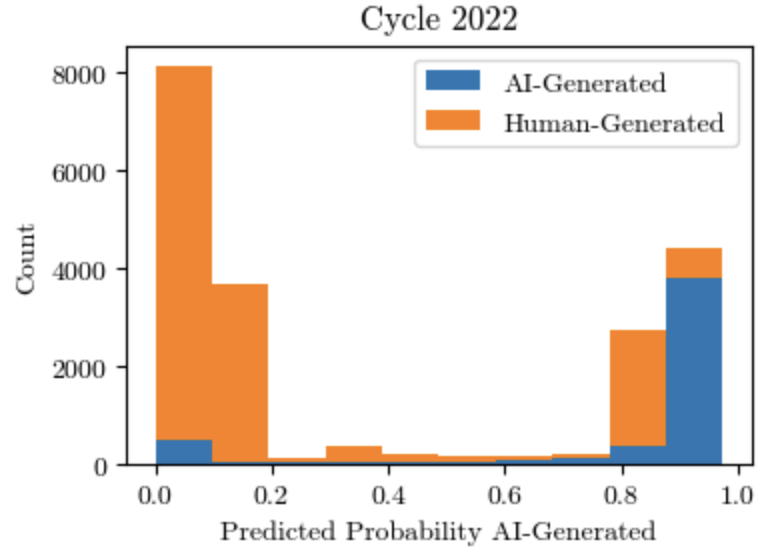
\includegraphics[width=0.4\textwidth]{figures/generative_ai/hist.png}
    \caption{Histogram of Uncalibrated GPTZero Scores, Cycle 2022}
    \label{fig:c2_hist}
\end{figure}

Figure \ref{fig:c2_hist} presents a histogram of uncalibrated GPTZero scores for the 2022 applicant-submitted and research-prompted, GPT-generated essays. Consistent with our knowledge that these essays were either entirely human-generated or entirely AI-generated, the histogram of values for $completely\_generated\_prob$ is bimodal. We see a large number of false positive essays with $completely\_generated\_prob \geq 0.8$. Similarly, Figure \ref{fig:c2_calibration} presents a calibration curve, which shows large differences between GPTZero's predicted probability and fraction of true positives in our data, proving that $completely\_generated\_prob$ is indeed not well-calibrated on our data. We thus perform statistic calibration on $completely\_generated\_prob$ to get an estimate of the probability that a given essay within our corpus is AI-generated (i.e., $\widehat{P(AI)}$) \cite{Niculescu-Mizil_Caruana_2005}.

\begin{figure}[tbh]
    \centering
    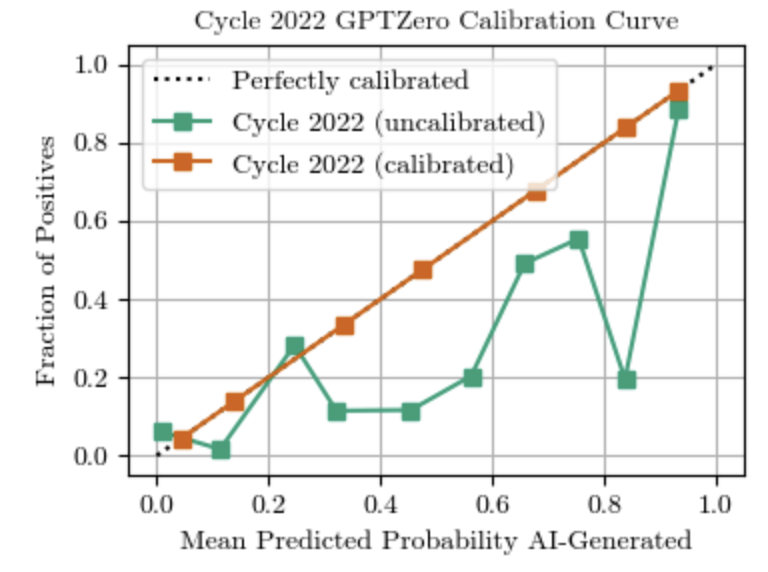
\includegraphics[width=0.4\textwidth]{figures/generative_ai/calibration.png}
    \caption{Calibration Curve of GPTZero's Predicted Probability AI-Generated, Cycle 2022}
    \label{fig:c2_calibration}
\end{figure}

With access to a large body of essays of known provenance ($15,149$ applicant-submitted Cycle 2022 essays and $5,002$ researcher-prompted ChatGPT-generated essays), we may use powerful calibration techniques comparing likelihood estimates to observed probabilities \cite{Zadrozny_Elkan_2002,Niculescu-Mizil_Caruana_2005}. Thus, we use isotonic calibration to calibrate GPTZero scores and produce $\widehat{P(AI)}$ \cite{Zadrozny_Elkan_2002}. We use this calibrated statistic in aggregate analyses and evaluate its utility according to its performance across all thresholds. I.e., we evaluate $\widehat{P(AI)}$ according to the area under its Receiver Operating Characteristic (ROC) curve (its ROC AUC score). We note that, in this case, a ROC AUC score of $0.5$ would indicate no discriminatory power, and a ROC AUC of $1.0$ would indicate perfect performance. We follow best practices in demanding an `acceptable' ROC AUC of at least $0.7$ \cite{Mandrekar_2010}.

\subsection{AI Detection In Lower-Stakes Decision-Making}
Finally, we are also interested in utilizing GPTZero outputs in lower-stakes decisions. This includes using these determinations to surface applicants who may require additional review or diligence, but extends also to determinations about an organisation's selection processes, pipeline, and outreach methods. Unlike in usage for automatic disqualification, this flag will only be used to draw additional selector attention to specific applications, and thus need not meet the $FPR \leq 0.02$ requirement. Instead, we focus on flagging application essays that are more likely to be AI-generated than not. That is, we use the threshold of $P(AI) \geq 0.5$ for this process. We opt to use this flag, rather than a raw probability, in analyses pertaining to an organisation's pipeline, as organisations often require more qualitative analysis of specific applications, and a binary indicator serves the secondary function of selecting these applications for us.

\section{Results}
\subsection{AI Detection In High-Stakes Decision-Making}\label{ssec:res_accuracy}
\subsubsection{The Veracity of AI Detection}
To determine how accurately we can identify AI-generated content, we compare the output statistic from our detector with actual knowledge of whether an essay was human- or computer-generated in Cycle 2022. We draw a ROC curve and report the area under that curve in Figure \ref{fig:c2_roc}. It does not matter here whether we use the calibrated or uncalibrated statistic, as the calibration process applies a monotonic transformation. The area under this ROC curve is an `outstanding' $0.91$, indicating good statistical power \cite{Mandrekar_2010}.

\begin{figure}[tbh]
    \centering
    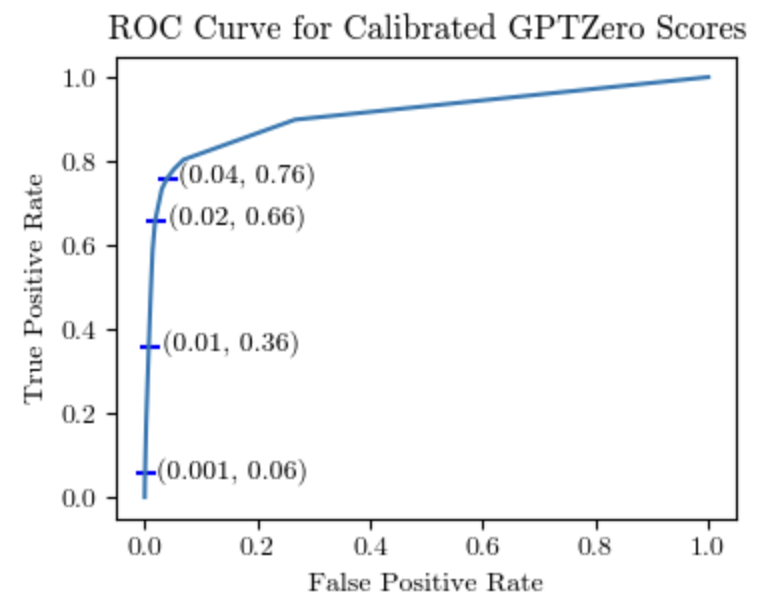
\includegraphics[width=0.4\textwidth]{figures/generative_ai/ROC.png}
    \caption{Receiver Operating Characteristic Curve of Calibrated GPTZero Scores, Cycle 2022}
    \label{fig:c2_roc}
\end{figure}

Despite good overall statistical power, GPTZero does not perform sufficiently well for the program to disqualify applicants on its basis alone. Section \ref{ssec:exp_accuracy} set a target of at least of $0.75$ TPR at $0.02$ FPR due to the program selecting only $2\%$ of completed applications. However, as Table \ref{tab:c2_tprs} shows (and as seen in Figure \ref{fig:c2_roc}), the threshold with a $2\%$ FPR identifies $66\%$ of AI-generated essays, leaving a third of such essays undetected and falling under our target of $0.75$ TPR.

\begin{table}[tbh]
   \centering
   \caption{Receiver Operating Characteristic AUC and Specificities, Cycle 2022}
   \label{tab:c2_tprs}
   \begin{tabular}{ l r }
       \toprule
       ROC AUC & $0.91$ \\
       TPR at $0.1\%$ FPR & $6\%$ \\
       TPR at $1\%$ FPR & $36\%$ \\
       TPR at $2\%$ FPR & $66\%$ \\
       TPR at $4\%$ FPR ($0.5$ Threshold) & $76\%$ \\
       \bottomrule\\
   \end{tabular}
\end{table}

\subsubsection{Heterogeneous Bias in AI Detection}
We next evaluate whether GPTZero is biased, on average, against genuine submissions from applicants with specific backgrounds. We conduct analyses of variance (ANOVAs) of the calibrated probability across gender and region categories in applicant-submitted essays from Cycle 2022 in Table \ref{tab:demo_anova}. As we know this data to be human-generated, this tests whether our detection method has heterogeneous false positive rates.

\begin{table}[htb]
    \centering
    \caption{Analysis of Variance for Calibrated Probability AI-Generated, Cycle 2022}
    \label{tab:demo_anova}
    \begin{tabular}{ l r r}
        \toprule
        Dimension & F Statistic & p Value \\
        \midrule
        Gender Identity & $41.4$ & $<0.01$ \\
        Region & $62.9$ & $<0.01$ \\
        \bottomrule\\
    \end{tabular}
\end{table}

\begin{table}[tbh]
    \centering
    \caption{Calibrated Probability AI-Generated and Inter-Cycle Changes by Applicant Demographics}
    \label{tab:demo_means}
    \begin{tabular}{ l r r r r r r}
        \toprule
        & \multicolumn{2}{c}{Cycle 2022} &  \multicolumn{2}{c}{Cycle 2023} & \multicolumn{2}{c}{Inter-Cycle T-Test} \\
        \cmidrule(lr){2-3} \cmidrule(lr){4-5} \cmidrule(lr){6-7}
        Demographic & Essays & $E(\widehat{P(AI)})$ & Essays & $E(\widehat{P(AI)})$ & t Score & p Value \\
        \midrule
        Male    & $6,475$ & $0.09$ & $11,080$ & $0.11$ & $8.63$ & $<0.01$ \\
        Female  & $8,710$ & $0.11$ & $13,380$ & $0.11$ & $-0.40$ & $0.69$ \\
        Other   & $176$   & $0.14$ & $355$    & $0.12$ & $-1.10$ & $0.27$ \\
        \midrule
        Caribbean               & $128$     & $0.17$ & $75$    & $0.15$ & $-0.47$ & $0.64$ \\
        ESEA     & $1,332$   & $0.13$ & $395$   & $0.13$ & $0.74$ & $0.46$ \\
        Five Eyes               & $522$     & $0.21$ & $1,865$ & $0.14$ & $-5.86$ & $<0.01$ \\
        Post-Soviet     & $85$      & $0.13$ & $705$   & $0.15$ & $0.59$ & $0.56$ \\
        South Asia     & $2,130$   & $0.08$ & $2,560$ & $0.09$ & $2.65$ & $0.01$ \\
        Latin America           & $709$     & $0.13$ & $2,855$ & $0.09$ & $-1.44$ & $0.15$ \\
        MENA   & $1,363$   & $0.11$ & $4,100$ & $0.12$ & $1.67$ & $0.09$ \\
        Subsahara      & $8,972$   & $0.09$ & $8,375$ & $0.09$ & $2.15$ & $0.03$ \\
        Other Europe            & $59$      & $0.20$ & $560$   & $0.12$ & $-2.75$ & $0.01$ \\
        Pacific Islands         & $5$       & $0.04$ & $0$      &  &  &  \\
        \midrule
        All         & $15,149$  & $0.10$ & $24,815$  & $0.11$ &  &  \\
        \bottomrule
    \end{tabular}
    % \begin{tablenotes}
    %     \small
    %     \item `Five Eyes' consists of Australia, Canada, New Zealand, the United Kingdom, and the United States.
    %     \item `MENA' stands for Middle East/North Africa.
    %     \item `ESEA' stands for East and Southeast Asia.
    %     \item $\widehat{E(P(AI))}$ is the mean estimated probability of essays being completely AI-generated.
    % \end{tablenotes}
\end{table}

Table \ref{tab:demo_anova} shows statistically significant variation across both dimensions in Cycle 2022. We therefore examine mean scores by gender identity and by countries of citizenship (grouped into larger categories). Column 3 of Table \ref{tab:demo_means} reports mean calibrated probabilities of being completely AI-generated for Cycle 2022 applicant submissions, which we know all predate ChatGPT. This shows that male applicants' essays receive lower estimates, on average, than applicants identifying as female or reporting some other gender category. While the magnitude of the difference is small, it raises the risk that using such scores in decision-making would bias outcomes against content genuinely created by women. Column 3 of Table \ref{tab:demo_means} also show genuinely human-generated applications from the Five Eyes – a group consisting of Australia, Canada, New Zealand, the United Kingdom, and the United States – get above average GTPZero scores. This is consistent with the fact that most large language models are trained primarily on texts from these countries, and may therefore align most closely with the style and lexical choices applicants from these countries use \cite{brown_language_2020}. However, as this bias appears to function in favor of non-native English speakers, it challenges previous work suggesting AI detectors are biased \textit{against} non-native English speakers \cite{liang_gpt_2023}.

\subsubsection{On Disqualifying Applicants via AI Detection}
We find here that no threshold meets our $FPR \leq 0.02$, $TPR \geq 0.75$ requirement for use in high-stakes decisions such as disqualifying candidates. Furthermore, we note that heterogeneous bias across a variety of demographic characteristics threaten to introduce biases into any process that uses this process to disqualify candidates. 

However, though we cannot meet the high bar of certainty required to disqualify a candidate, we may still be able to aggregate this information to yield valuable cohort-level insights, and may also use this information for lower-stakes decision-making (such as flagging a candidate for manual review).

\subsection{AI Detection in Aggregate Statistics}\label{ssec:res_statistics}
\subsubsection{The Analytic Utility of GPTZero}
Recall that the area under $\widehat{P(AI)}$'s ROC curve in Figure \ref{fig:c2_roc} is an `outstanding' $0.91$ (see: Table \ref{tab:c2_tprs}) \cite{mandrekar_receiver_2010}. This far exceeds our requirement of $0.80$ laid out in Section \ref{ssec:exp_statistics}, indicating that $\widehat{P(AI)}$ performs well at a variety of thresholds, and that use of this statistic in aggregate analysis will yield valuable results. 

We note as a caveat that our $\widehat{P(AI)}$ exhibits heterogeneous bias across demographic groups. Thus, analyses comparing GPTZero scores across different demographic subgroups risk conflating genuine difference in generative AI usage with measurement biases. We therefore focus primarily on analysing within-group changes in $\widehat{P(AI)}$.

\subsubsection{Applicants' Potential Use of AI-Generated Content}
We focus our subsequent analysis primarily on the potential use of generative AI by applicants in Cycle 2023. We note here that the mean probability of an essay being AI-generated within a corpus is exactly the expected proportion of AI-generated content within that corpus. Thus, we test for changes in mean $\widehat{P(AI)}$. Table \ref{tab:demo_means} presents mean $\widehat{P(AI)}$ for 2023 (column 3) and 2022 (column 5), as well as test statistics of whether there is a difference in means (columns 6 and 7).

\begin{table*}[tbh]
    \centering
    \caption{ANOVA for differences in GPTZero Detection Scores by Partners, Cycle 2023 }
    \label{tab:c3_partner_anova}
    \begin{tabular}{ l r r r r }
        \toprule
        \multicolumn{3}{c}{} & \multicolumn{2}{c}{ANOVA Results} \\
        \cmidrule(lr){4-5}
        Referring Partner & Essays & Share `AI-Generated' & F Statistc & p Value \\
        \midrule
        Partner A & $540$ & $0.041$ & $0.064$ & $0.80$ \\
        Partner B & $390$ & $0.044$ & $0.004$ & $0.95$ \\
        Partner C & $325$ & $0.049$ & $0.320$ & $0.57$ \\
        Partner D & $315$ & $0.029$ & $1.599$ & $0.21$ \\
        Partner E & $235$ & $0.064$ & $2.526$ & $0.11$ \\
        Partner F & $205$ & $0.039$ & $0.076$ & $0.78$ \\
        Partner G & $170$ & $0.047$ & $0.071$ & $0.79$ \\
        Partner H & $150$ & $0.027$ & $0.970$ & $0.33$ \\
        Partner I & $150$ & $0.007$ & $4.829$ & $0.03$ \\
        Partner J & $135$ & $0.022$ & $1.415$ & $0.23$ \\% suppressing to save space
        \midrule
        All Submissions & $24,815$ & $0.040$ & \\
        \bottomrule
    \end{tabular}
    % \begin{tablenotes}
    %     \small
    %     \item Share `AI-Generated' is the share of essays identified as more likely to be AI-generated than not.
    %     \item 
    % \end{tablenotes}
\end{table*}

We find statistically significant increases in the $\widehat{P(AI)}$ for only two overlapping subgroups: male applicants and applicants from the Indian subcontinent. In both cases the magnitude of the increase is small, suggesting that at least in Cycle 2023, the use of generative AI was limited. However, other findings preclude interpreting this change as a direct measure of increased generative AI use. In two regions, the Five Eyes and Europe (excluding the United Kingdom and former Soviet Union), we found a statistically significant decrease in the calibrated estimated probability that essays were completely AI generated. Since we can assume very few (if any) applicants in Cycle 2022 had access to generative AI, this cannot be interpreted as a decrease in AI use. It may instead be that both regions' high average scores in 2022 were a fluke of the cohort, and that these regions reverted to the mean in 2023. Alternatively, it is possible that, in these regions, Cycle 2023 applicants used AI detection tools to ensure that their content would not be flagged by our detector (although this would require such detector usage to offset any actual generative AI use) \cite{gptzero_gptzero_2023}. In either case, this analysis surfaces interesting discrepancies demanding further interrogation in future application cycles. 

\subsection{AI Detection In Lower-Stakes Decision-Making}
\subsubsection{Flagging Applicants Likely to Have Used Generative AI}\label{ssec:flags}
In Cycle 2023 decision-making, our partner program used GPTZero's AI detection to ``flag'' applicants that we believe are likely to be AI-generated. As previously mentioned, we do not have sufficient confidence in the statistical power of fairness of any determination we could make to disqualify applicants for possible generative AI usage. We have set a high bar for such confidence. However, we might still use these flags to direct human reviews of application essays, or to evaluate our application pipeline.

For this process, we use a cutoff of $0.5$ on our calibrated predictor, meaning that essays flagged as `AI-Generated' are more likely than not to be so ($\widehat{P(AI)} \geq 0.5$). This threshold is shown in Table \ref{tab:c2_tprs} with a true positive rate of $76\%$ and a false positive rate of $4\%$.

In practice, the program used these flags throughout Cycle 2023 to direct the attention of human reviewers towards essays that were likely to be AI-generated. We note that the program did not ban the usage of generative AI, so these applicants were not penalised for these determinations. However, generative AI's tendencies towards plagiarism are well-documented, and the program did devote additional attention towards catching plagiarism in flagged applicants \cite{dehouche_plagiarism_2021}.

\subsubsection{Evaluating Partners with AI Detection}
Talent identification programs are perennially interested in reaching talent across their target demographic. Our partner program employs an outreach strategy of cultivating relationships with `referring partners', i.e., organisations that encourage and support applicants. Relevant applicants are attributed to referring partners based on the custom links applicants use to reach the program's website, as well as questions in the application form about how applicants learned of the program.

As these partnerships form a large portion of the program's outreach, the program regularly evaluates the utility of this approach. As part of this evaluation, the program evaluates the likelihood of irregular generative AI usage in the essays associated with the program's referring partners. Evidence that any of the referring partners used generative AI to create large volumes of applications would warrant further investigation before continuing said partnerships.

For this evaluation, we associate flagged essays with the appropriate referring partners. For the purposes of this paper and to preserve the program's anonymity, we have limited this analysis to the partners with the most essays and have hidden individual partners' identities. We then conduct an ANOVA to test for variations in the frequency of flagged essays by partner. Table \ref{tab:c3_partner_anova} shows the results of this ANOVA.

Here, only one of the partners studied was associated with essays identified as AI-generated at a rate meaningfully different from the overall pool. However, the partner in question, Partner I, was actually associated with fewer essays than average identified as AI-generated. This may be driven by the (Africa-based) partner working primarily with demographics identified in Cycle 2022 analyses as naturally having below-average calibrated scores. Overall, the program found no evidence of generative AI usage associated with any particular partner, which served as an important step in validating program involvement with these partners.

\section{Discussion}\label{sec:conc}
Our natural experiment on Cycle 2022 data enjoyed optimal conditions for AI detection; the synthetic essays were not paraphrased or edited, and all of the human-written essays were real submissions to the program. Despite this, at sensitivity levels comparable to acceptance rates into selective programs, we do not achieve high specificity. Thus, we conclude that the program should not use this technology in making high-stakes decisions such as disqualifying candidates. Furthermore, we find heterogeneous biases in our detection of AI essays. We do, however, see good overall statistical power. Therefore, we find utility in using AI detection for aggregate analyses, so long as these analyses account for the risk of heterogeneous biases. We demonstrate one such analysis on data supplied by the program: examining the potential scale of AI usage by demographic group. Finally, we note that organisations may still use determinations in making lower-stakes decisions such as the direction of additional selector scrutiny and post-hoc evaluation of application pathways. We conclude that organisations looking to assess the use of generative AI in essays they receive have an opportunity to do so with GPTZero or other AI detection tools.

This analysis is limited in scope to only one method for AI generation and one method for identification of that generation. Thus, our present results are limited to these methods. One avenue for future analyses include using other methods of essay generation and AI detection and seeking out differential performance on essays in response to particular prompts. In particular, we intend further work to focus on understanding the effect of paraphrasing software on our results, as the paraphrasing of generative AI outputs has been shown to render them less detectable \cite{mitchell_detectgpt_2023,kalpesh_krishna_paraphrasing_2023}.

Furthermore, the work with our partner program is longitudinal and ongoing, and our partner program is presently administering application Cycle 2024. We intend to incorporate the 2024 application cycle into our analyses going forward, and to further extend this with subsequent application cycles.
% \begin{savequote}[8cm]
% Alles Gescheite ist schon gedacht worden.\\
% Man muss nur versuchen, es noch einmal zu denken.

% All intelligent thoughts have already been thought;\\
% what is necessary is only to try to think them again.
%   \qauthor{--- Johann Wolfgang von Goethe \cite{von_goethe_wilhelm_1829}}
% \end{savequote}

\chapter{\label{ch:discussion}Discussion}

\minitoc

\section{Implications and Recommendations}
Here we analyse the implications of using IAIDSTs in talent identification. We first look at the strengths and limitations of post-hoc explanations and prescribe appropriate use cases for these types of IAIDSTs. Second, we examine the strengths and weaknesses of intrinsically interpretable models, including purpose-built models, and make similar prescriptions. Finally, we distil our insights in purpose-building IAIDSTs for TI professionals and extrapolate to general recommendations.

\section{Limitations and Future Work}
We note the limitations of this research method. We examine first limitations of individual case studies and note how other methodologies might address these limitations. We then raise concerns about our research's external validity, especially with regard to our recommendations and prescriptions. We address these concerns and note ways in which this research should not be used. Finally, we highlight areas in which researchers may continue this work or expand upon it.

\section{Conclusion}
To-do

%%%%% APPENDICES
% Starts lettered appendices, adds a heading in table of contents, and adds a
%    page that just says "Appendices" to signal the end of your main text.
\startappendices
% Add or remove any appendices you'd like here:
% \begin{savequote}[8cm]
% \textlatin{Cor animalium, fundamentum e\longs t vitæ, princeps omnium, Microco\longs mi Sol, a quo omnis vegetatio dependet, vigor omnis \& robur emanat.}

% The heart of animals is the foundation of their life, the sovereign of everything within them, the sun of their microcosm, that upon which all growth depends, from which all power proceeds.
%   \qauthor{--- William Harvey \cite{harvey_exercitatio_1628}}
% \end{savequote}

\chapter{\label{app:terminology}Definitions and Terminology}

\minitoc

\section{To-do}
To-do
% \begin{savequote}[8cm]
% \textlatin{Cor animalium, fundamentum e\longs t vitæ, princeps omnium, Microco\longs mi Sol, a quo omnis vegetatio dependet, vigor omnis \& robur emanat.}

% The heart of animals is the foundation of their life, the sovereign of everything within them, the sun of their microcosm, that upon which all growth depends, from which all power proceeds.
%   \qauthor{--- William Harvey \cite{harvey_exercitatio_1628}}
% \end{savequote}

\chapter{\label{app:misleadingexplanations}Reference Materials for Misleading Explanations of AI Outputs in Talent Identification}

\minitoc

\section{Tasks}\label{sec:tasks}
Rather than an evaluation of a machine (where a user might rate a model as being correct because it is consistent), we restrict our analysis to human-in-the-loop tasks (where, if a user disagrees with a machine, they might override it) to better simulate and assess the sense in which a human-in-the-loop is \emph{vulnerable} to being mislead by an explanation.

Furthermore, we recognize that in many cases, a user's confidence in their own judgement would crowd out any possible effect of the AI system (and any associated explanation), or the ambiguity about whether any ground truth exists at all may lead a user to hold steadfast in their opinions. Thus, we avoid domains like ``is this an image of a cat?'' where it is obvious to the human whether the image is one of a cat. Similarly, we avoid tasks without a clear ground truth such as ``is this language offensive?'' or ``is this a good work of art?''. (Philosophers continue to argue whether or not these questions have objective answers. Kant, for example, contended that, while they do not admit objective answers, subjects are nonetheless justified in making universal claims \cite{zangwill_aesthetic_2023}.)

\begin{figure*}[htbp]
    \hspace{\fill}
    \subfloat[\label{survey_table_adult}]{
        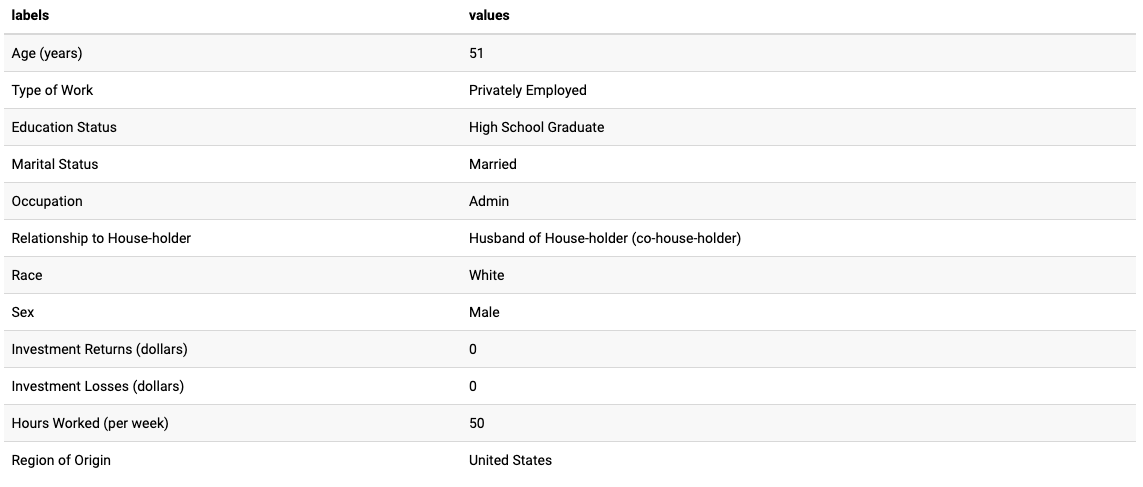
\includegraphics[clip, width=0.4\textwidth]{figures/misleading_explanations/survey_table_adult.png}}
    \hspace{\fill}
    \subfloat[\label{survey_table_credit} ]{
        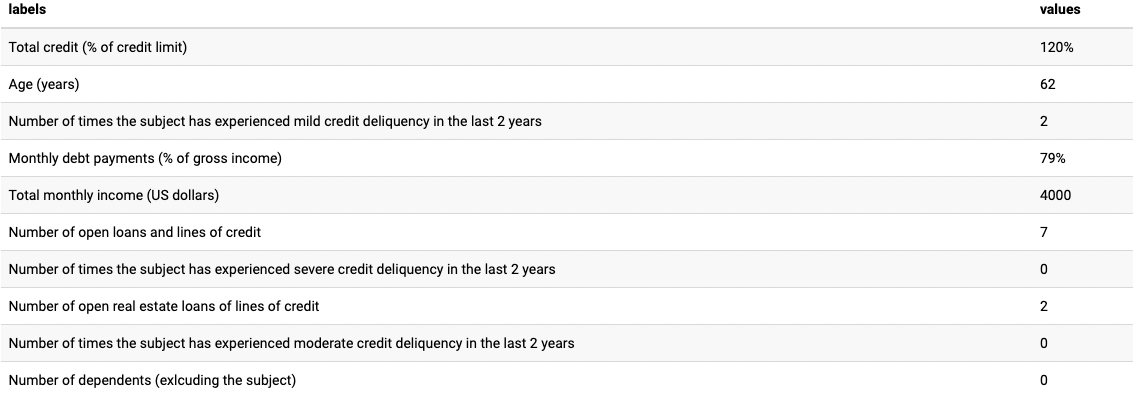
\includegraphics[clip, width=0.4\textwidth]{figures/misleading_explanations/survey_table_credit.png}}
    \hspace{\fill}
    \caption{Features from a Sample Case in (a) the Salary Estimation and (b) the Credit Prediction Tasks}
    \label{fig:survey_table}
\end{figure*}

\begin{figure*}[htbp]
    \hspace{\fill}
    \subfloat[\label{survey_pred_adult}]{
        
\includegraphics[clip, width=0.4\textwidth]{figures/misleading_explanations/survey_prediction_adult.png}}
    \hspace{\fill}
    \subfloat[\label{survey_pred_credit} ]{
        
\includegraphics[clip, width=0.4\textwidth]{figures/misleading_explanations/survey_prediction_credit.png}}
    \hspace{\fill}
    \caption{Predictions from a Sample Case in (a) the Salary Estimation and (b) the Credit Prediction Tasks}
    \label{fig:survey_pred}
\end{figure*}

We choose two standard benchmark datasets: Adult and Give Me Some Credit \cite{kohavi_scaling_1996,GiveMeSomeCredit}. We choose these because such datasets are typically the grounds on which xAI methods are developed and critiqued. The Adult dataset specifically has been used as a benchmark in multiple xAI studies, including \textcite{weerts_case-based_2019}, \textcite{weerts_human-grounded_2019}, and \textcite{ribeiro_anchors_2018}. Various credit datasets, including Give Me Some Credit, are common as benchmarks in xAI studies like \textcite{bansal_does_2021}, \textcite{ustun_learning_nodate}, and \textcite{krishna_disagreement_2022}.

The dependent variable (to be estimated by the participant) of the Adult dataset is ``Does this person make more than \$50,000?''. However, we adjusted the amount due to inflation (this amount in 1994 is roughly \$100,000 today). Thus, we ask ``Does this person make more than \$100,000?''. The dependent variable of the Give Me Some Credit dataset is ``Will this person be at least 90 days delinquent on a credit payment in the next two years'', which we simplify to ``Will this person experience severe credit delinquency in the next two years'' (we also include a definition of ``severe credit delinquency'').

The participant has access to a table containing all data the model does in both cases; samples of these tables are shown in Figure \ref{fig:survey_table}. Figure \ref{fig:survey_pred} displays the initial estimate of the AI system for the very same samples, as they are shown to participants.

\section{Questions and Constructs}\label{sec:constructs}

We ask three questions both before and after explanation. In the Salary Estimation task, we ask ``How much money do you estimate this person makes?'', to which the possible responses are ``Less than \$100,000 per year'' and ``More than \$100,000 per year''. In the Credit Prediction task, we ask ``Do you predict that this person will experience severe credit delinquency?'', where the answers are ``Will not experience severe delinquency'' and ``Will experience severe delinquency''. In either case, this yields a binary $estimate$ variable. 

Then, we ask ``How confident are you in your estimation?'', which has a 20-point sliding scale of possible responses. This yields the $confidence$ (confidence) variable with a value between $1$ and $20$. 

Finally, we ask ``How much do you trust the AI system's estimation?'', which has a 20-point sliding scale of possible responses. This yields the attitudinal trust variable, $trust_{attitude}$, also with a value between $1$ and $20$. 

\begin{figure*}[htbp]
    \centering
    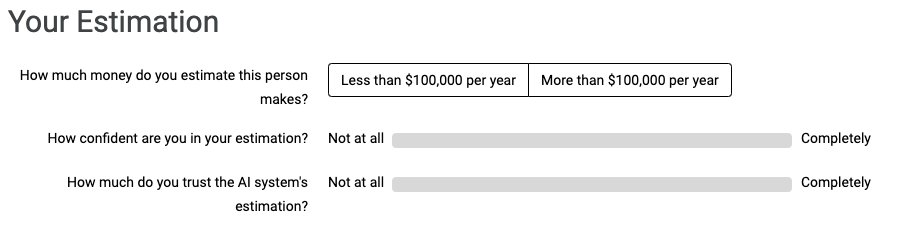
\includegraphics[width=0.8\textwidth]{figures/misleading_explanations/survey_question_adult.png}
    \caption{Three Questions Asked Twice per Case (Salary Estimation)}
    \label{fig:survey_question_adult}
\end{figure*}

\begin{figure*}[htbp]
    \centering
    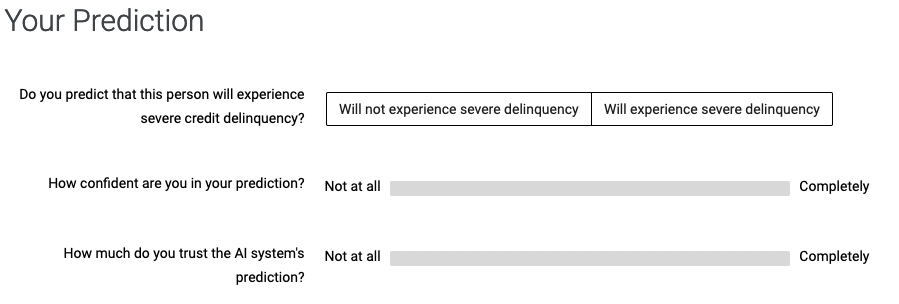
\includegraphics[width=0.8\textwidth]{figures/misleading_explanations/survey_question_credit.png}
    \caption{Three Questions Asked Twice per Case (Credit Prediction)}
    \label{fig:survey_question_credit}
\end{figure*}

These three questions are asked twice; once before the participant sees one of the three experimental conditions (SHAP, Anchors, and Confidence), and once again after. We index the `before' case as $before$ and the `after' case as $after$. 

Thus, we collect six variables from participants per case: $estimate^{before}$, $confidence^{before}$, $trust_{attitude}^{before}$, $estimate^{after}$, $confidence^{after}$, $trust_{attitude}^{after}$. The presentation of the three questions is shown in Figures \ref{fig:survey_question_adult} and \ref{fig:survey_question_credit}.

We also collect two additional variables per case: $answer$ and $recommendation$. In each case, $answer$ is the correct output for the case (as in our test output data), and $recommendation$ is the machine's recommendation of what the user should estimate for that case. 

We can now define some constructed variables for use in our analysis. First, we define a $agreement$ to be whether the user's estimate is in agreement with the machine's recommendation in Equation \ref{eq:trimp_agreement}. 

\begin{equation}
    agreement^x := estimate^x == recommendation
    \label{eq:trimp_agreement}
\end{equation}

We now define a variable $trust_{behaviour}$ in Equation \ref{eq:trimp}, which is a combination of the $estimate$, $confidence$, and $agreement$ variables to yield a $40$-point scale of behavioural trust. Here, $-19$ is absolute confidence that the system is wrong and $20$ is absolute confidence that the system is right. Let:

\begin{equation}
    trust_{behaviour}^x := \left\{
        \begin{array}{ll}
            confidence^x & \quad agreement^x\\
            1 - confidence^x & \quad otherwise
        \end{array}
    \right.
    \label{eq:trimp}
\end{equation}

In order to reason about the change in a variable due to the explanation, we define `$\Delta$' constructs as the difference between after- and before-explanation for each variable, as seen in Equation \ref{eq:deltas}.

\begin{equation}
    \Delta x := x^{after} - x^{before}
    \label{eq:deltas}
\end{equation}

Informally, $\Delta trust_{attitude}$ is the effect of the explanation on the participant's attitudinal trust in the AI determination. Formally, $\Delta trust_{attitude} := trust_{attitude}^{after} - trust_{attitude}^{before}$. E.g., suppose a participant sees a determination they believe to be incorrect in the absence of an explanation, they might express distrust in that system and rate their trust low (say $3$); suppose further that, the explanation provided is persuasive, and the participant rates their trust high (say $19$) after reading it; the $\Delta trust_{attitude}$ for this case would be $19 - 3 = 16$.

\section{Models}\label{sec:models}
In this study, we rely on three different models. We use a random forest classifier as our base model. We use a SHAP explainer to produce one of our explanatory conditions, and a Scoped Anchors explainer to produce another (our final explanatory condition is produced natively by the random forest). 

We opt for a random forest model as they are still ubiquitous in the field of AI, and the Adult and Give Me Some Credit datasets lack the kind of feature richness required to noticeably benefit from more sophisticated model architectures \cite{Grinsztajn_Oyallon_Varoquaux_2022}. The random forest classifiers classify points in each data set into either of the two outcome conditions. Our random forest classifier achieves 86\% test accuracy on the Adult dataset and 93\% test accuracy on the Give Me Some Credit dataset.

\begin{figure*}[htbp]
    \hspace{\fill}
    \subfloat[\label{survey_shap_adult}]{
        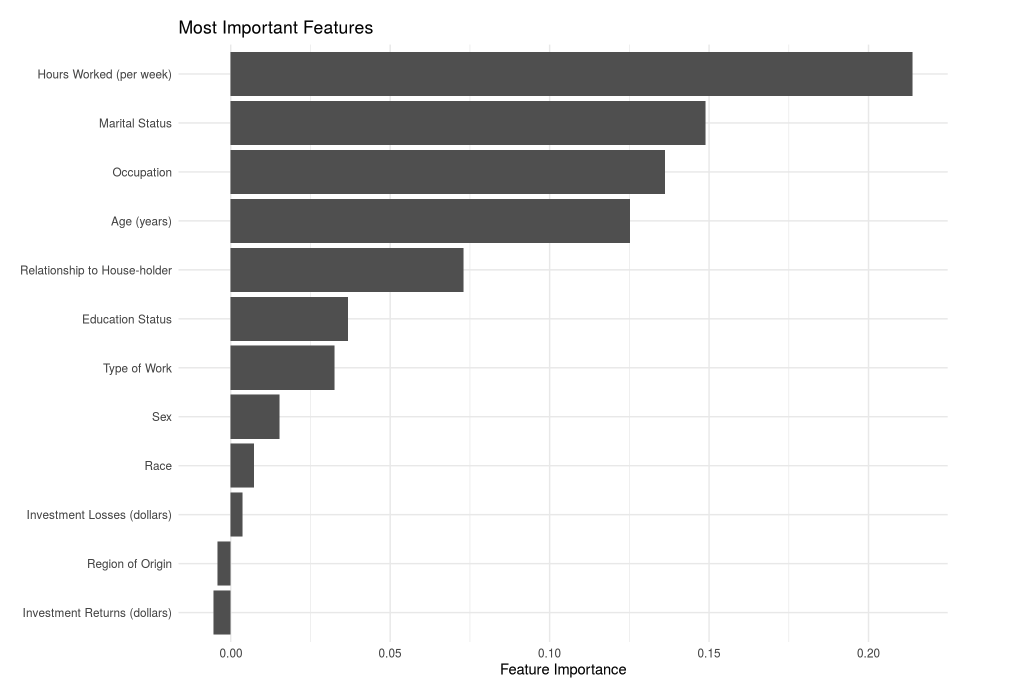
\includegraphics[clip, width=0.4\textwidth]{figures/misleading_explanations/survey_shap_adult.png}}
    \hspace{\fill}
    \subfloat[\label{survey_shap_credit} ]{
        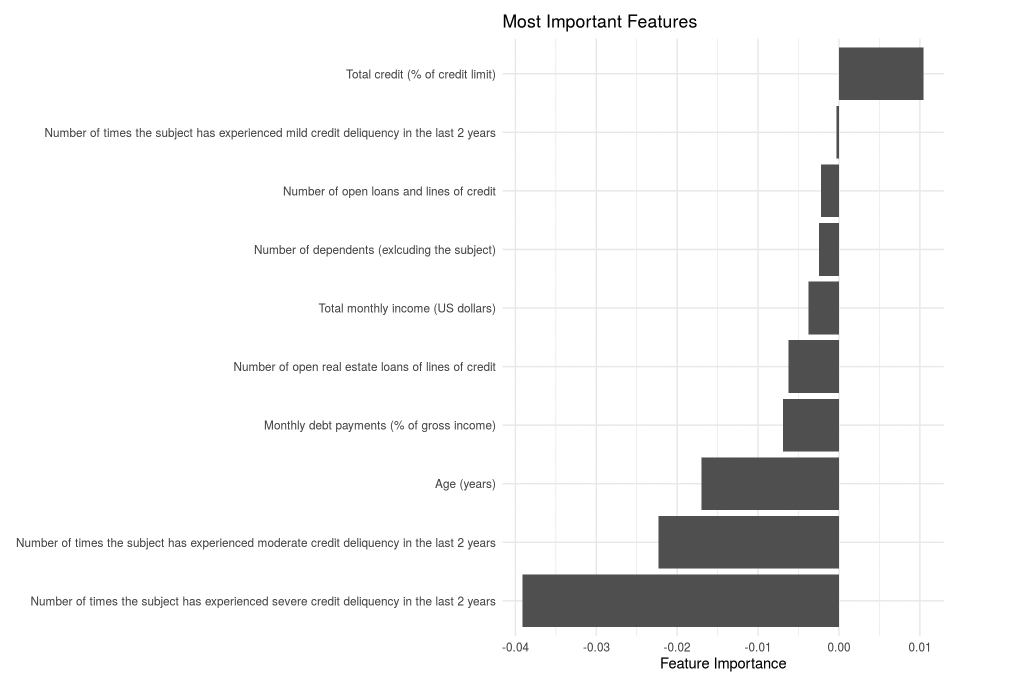
\includegraphics[clip, width=0.4\textwidth]{figures/misleading_explanations/survey_shap_credit.png}}
    \hspace{\fill}
    \caption{Sample SHAP Explanations in (a) the Salary Estimation and (b) the Credit Prediction Tasks}
    \label{fig:survey_shap}
\end{figure*}

\begin{figure*}[htbp]
    \hspace{\fill}
    \subfloat[\label{survey_anchor_adult}]{
        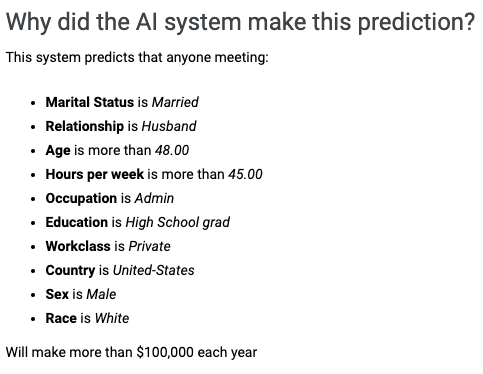
\includegraphics[clip, width=0.4\textwidth]{figures/misleading_explanations/survey_anchor_adult.png}}
    \hspace{\fill}
    \subfloat[\label{survey_anchor_credit} ]{
        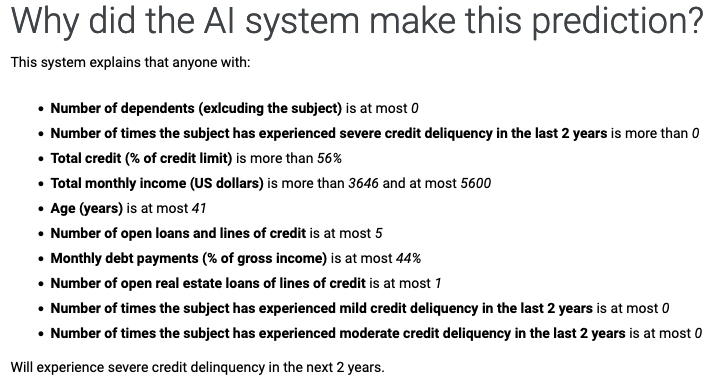
\includegraphics[clip, width=0.4\textwidth]{figures/misleading_explanations/survey_anchor_credit.png}}
    \hspace{\fill}
    \caption{Sample Anchors Explanations in (a) the Salary Estimation and (b) the Credit Prediction Tasks}
    \label{fig:survey_anchor}
\end{figure*}

\begin{figure*}[htbp]
    \hspace{\fill}
    \subfloat[\label{survey_confidence_adult}]{
        
\includegraphics[clip, width=0.4\textwidth]{figures/misleading_explanations/survey_confidence_adult.png}}
    \hspace{\fill}
    \subfloat[\label{survey_confidence_credit} ]{
        
\includegraphics[clip, width=0.4\textwidth]{figures/misleading_explanations/survey_confidence_credit.png}}
    \hspace{\fill}
    \caption{Sample Confidence Explanations in (a) the Salary Estimation and (b) the Credit Prediction Tasks}
    \label{fig:survey_confidence}
\end{figure*}

Our three explanatory conditions are: SHAP, Anchors, and Confidence. SHAP explanations show participants a plot of feature importances, where the presented importances are the Shapley Values calculated for each feature. In the Anchors explanations, participants are shown rules that nearly guarantee that other cases following these rules will have the same estimate. In the Confidence condition, participants are shown the model's confidence in its estimate (based on the average output of all decision trees in the random forest model). We expect that providing any of these three explanations will generate an increase in trust even when the AI system is incorrect.

We select these three conditions carefully. We wish to test the popular feature importance explanation methods, of which SHapley-based Additive exPlanations, or SHAP (the `SHAP' condition), is a prominent example \cite{lundberg_unified_2017}. These explanations weight the importances of different features in a particular prediction. They are are often used to highlight aspects of the model to users and have been criticised in \textcite{kumar_problems_2020} for failing to follow norms of explanations drawn from philosophy, psychology, and cognitive science, making them bad candidates for explanation to end users. We also test the Scoped Anchors explanation algorithm (the `Anchors' condition) \cite{ribeiro_anchors_2018}. These explanations justify individual model predictions following human-centred norms by providing rules that bound model behaviour. \textcite{bansal_does_2021} and \textcite{jacobs_how_2021} both note that this styles of explanation raises user trust in a model. Finally, we also test the provision of the model's own confidence in its estimate (the `Confidence' condition). While confidence statistics are not generally regarded as an xAI method, they serve a similar function in that they indicate to the user something about the model's operation which allows evaluation of the model on those grounds.

We fine-tuned the visual design of each condition with a pilot study using the Adult dataset. In the pilot, we asked participants to indicate which of a range of visualisations is the most intuitive, and asked various questions to test their comprehension. For the SHAP condition, we found that a bar plot plotting feature importances, a format used for all feature importance methods across the field, appeared to be considered more intuitive \cite{weerts_human-grounded_2019}. As both models have relatively few features, we opted to show all features. For the Anchors condition, we found that a verbal explanation of the Anchors, mimicking formats used by popular social media platforms, was considered the most intuitive \cite{ribeiro_anchors_2018}. The formats used in the study itself can be seen in Figures \ref{fig:survey_shap}, \ref{fig:survey_anchor}, and \ref{fig:survey_confidence}.

\section{The Study}\label{sec:study}
We collected data in surveys designed and hosted on Formr.\footnote{www.formr.org} The participants were recruited via Prolific Academic's standard sampling method restricted to the United States (to match the origin of both datasets).\footnote{www.prolific.co}

Participants completed the study 6 times with 6 cases drawn from a pool of 39, where the AI system is correct on 20 out of the 39. To avoid learned effects related to the accuracy of either the model or the sample pool, participants were not told the machine accuracy or the distribution of the case pool. No participants were permitted to take part in both studies.
% \begin{savequote}[8cm]
% \textlatin{Cor animalium, fundamentum e\longs t vitæ, princeps omnium, Microco\longs mi Sol, a quo omnis vegetatio dependet, vigor omnis \& robur emanat.}

% The heart of animals is the foundation of their life, the sovereign of everything within them, the sun of their microcosm, that upon which all growth depends, from which all power proceeds.
%   \qauthor{--- William Harvey \cite{harvey_exercitatio_1628}}
% \end{savequote}

\chapter{\label{app:chatgptgeneration}ChatGPT Generation}

\minitoc

\section{To-do}
To-do
% \begin{savequote}[8cm]
% \textlatin{Cor animalium, fundamentum e\longs t vitæ, princeps omnium, Microco\longs mi Sol, a quo omnis vegetatio dependet, vigor omnis \& robur emanat.}

% The heart of animals is the foundation of their life, the sovereign of everything within them, the sun of their microcosm, that upon which all growth depends, from which all power proceeds.
%   \qauthor{--- William Harvey \cite{harvey_exercitatio_1628}}
% \end{savequote}

\chapter{\label{app:spfproofs}Proofs for the SPF Theorem}

\minitoc

\section{Proof of Greedy Approximation}
Here, we prove that the greedy approximation method introduced in Algorithm \ref{alg:frontier} for SPF is a $(1-\frac{1}{e})$-approximation for our standard class of diversity functions subject to a cardinality constraint.

Recall that a diversity function $f: 2^X -> \mathbb{R}^+$  maps a cohort (a set of applicants) to a ``diversity score'' (a non-negative real number). Here, our applicant pool $X$ is represented as a set with applicants as its members, and possible cohorts $C \subseteq X$ are subsets of $X$. We restrict our analysis to standard diversity functions, which we assert are monotonic ($A \subseteq B -> f(A) \leq f(B)$) and submodular ($A \subseteq B \and x \notin B -> f_A(x) \geq f_B(x)$ (here, $f_S(e) = f(S \cup \{e\}) - f(S)$ denote the marginal gain of adding element $e$ to set $S$) .We demonstrate elsewhere that many common understandings of diversity are represented by standard diversity functions.

We now recreate a proof of Theorem \ref{thm:greedy-approximation} first demonstrated in \cite{nemhauser_analysis_1978}.

\begin{theorem}\label{thm:greedy-approximation}
    Let $(S_0...S_k)$ be a sequence of sets where $S_0$ is the empty set and $S_{i>0}$ is defined by following Algorithm \ref{alg:frontier}. Further, let $O := argmax_S(f(S) : |S| = k)$ be the set of size $k$ that maximizes $f$. Then $f(S_k) \geq (1 - \frac{1}{e})f(O)$. 
\end{theorem}

\emph{Proof}. Let ${o_1...o_k} = O$ be any ordering of the elements of $O$. Let ${s_i} := S_i - S_{i-1}$ be the element added to $S_{i-1}$ to form $S_i$.

By monotonicity, we have $\forall i . f(O) \leq f(O \cup S_i)$.  We can then write $f(O \cup S_i) = f(O \cup S_i) - f(S_i) + f(S_i) = \sum_{j=1}^{k} \bigl f(S_i \cup {o_1...o_j}) - f(S_i \cup {o_1...o_{j-1}}) \bigr$. I.e., $f(O \cup S_i) = f(O \cup S_i) - f(S_i) + f(S_i) = \sum_{j=1}^{k} f_{S_i \cup {o_1...o_{j-1}}}(o_j)$.

By submodularity, $\forall j \in [1...k] . f_{S_i \cup {o_1...o_{j-1}}}(o_j) \leq f_{s_i}(o_j)$. Thus, $f(O) \leq f(S_i) + k*f_{S_i}(s_{i+1})$. 

Since Algorithm \ref{alg:frontier} guarantees that $\forall e \in X - S_i . f_{S_i}(e) \geq f_{S_i}(e)$, it follows that, at every stage, $f(S_{i+1}) - f(S_i) \geq \frac{1}{k} \bigl f(O) - f(S_i) \bigr$. 

Then induction yields $f(O) - f(S_k) \leq {\bigl 1 - \frac{1}{k} \bigr}^k f(O) \leq \frac{1}{e} f(O)$.

%%%%% REFERENCES

% JEM: Quote for the top of references (just like a chapter quote if you're using them).  Comment to skip.
% \begin{savequote}[8cm]
% The first kind of intellectual and artistic personality belongs to the hedgehogs, the second to the foxes \dots
%   \qauthor{--- Sir Isaiah Berlin \cite{berlin_hedgehog_2013}}
% \end{savequote}

\setlength{\baselineskip}{0pt} % JEM: Single-space References

{\renewcommand*\MakeUppercase[1]{#1}%
\printbibliography[heading=bibintoc,title={\bibtitle}]}


\end{document}
